\documentclass[11pt,a4paper]{article}
\usepackage[utf8]{inputenc}\usepackage[T1]{fontenc}\IfFileExists{italian.ldf}{\usepackage[italian]{babel}}{\usepackage[english]{babel}}
\usepackage{amsmath,amssymb,amsthm,geometry,hyperref,tikz}\geometry{margin=22mm}
\newcommand{\R}{\mathbb R}\newcommand{\N}{\mathbb N}\newcommand{\pagina}[1]{\clearpage}
\newcommand{\nota}[1]{\par\textit{Nota di trascrizione: #1}\par}
\setlength{\emergencystretch}{2em}
\begin{document}\begin{center}{\LARGE Analisi 2}\\Trascrizione degli appunti\end{center}
\nota{Le formule vengono mantenute anche quando negli appunti risultano incomplete; eventuali problemi sono segnalati.}
% Pagina originale 1
\pagina{1}\section*{Legenda}
\subsection*{1. Integrali impropri (o generalizzati)}
Convergenza e divergenza; integrazione a valor principale; osservazioni sull'integrazione a V.P.; esempi fondamentali; osservazione sulla divergenza basata sugli asintoti orizzontali; 1: $f(x)\ge0\Rightarrow F(x)$ crescente monotona; 2: teorema del confronto; 3: teorema del confronto asintotico; confronto con il valore assoluto; $f$ assolutamente integrabile.
\subsection*{2. Funzioni a più variabili}
Topologia euclidea; proprietà della distanza; intorno sferico o palla di $x_0$; osservazioni sulla distanza; punto di accumulazione; palla bucata; limite; caratterizzazione del limite in una funzione a valori vettoriali; convergenza e divergenza; continuità; punto isolato; continuità nei limiti; teorema ponte; osservazioni e applicazioni sull'esistenza di un limite; funzioni omogenee; continuità delle funzioni composte; proiezione canonica; disuguaglianza di Cauchy-Schwartz; teorema del doppio confronto; $|f(x)|\xrightarrow{x\to x_0}0\iff f(x)\xrightarrow{x\to x_0}0$; insieme aperto; insieme chiuso; non aperto $\not\Rightarrow$ chiuso; frontiera o bordo; chiusura di un insieme; insieme limitato; massimo e minimo; insieme compatto; teorema sulla compattezza (insieme compatto $\iff$ insieme sequenzialmente compatto); 4: teorema di Weierstrass; 5: una funzione continua trasforma compatto in compatto; $B$ aperto/chiuso $\Rightarrow f^{-1}(B)$ aperto/chiuso; unioni e intersezioni tra insiemi aperti/chiusi; insieme convesso; insieme connesso per archi; convesso $\Rightarrow$ connesso per archi; 6: teorema degli zeri per $\R^n$; $f$ trasforma connessa in connessa.
\subsection*{3. Rapporto incrementale}
Gradiente; jacobiano e matrice jacobiana; differenziabilità.
% Pagina originale 2
\pagina{2}
Miglior approssimazione lineare; 7: differenziabilità $\Rightarrow$ continuità; cos'è la mappa lineare $L_{x_0}$; 8: differenziabilità $\Rightarrow\exists J_f\wedge A_{x_0}=J_f(x_0)$; 9: differenziabilità $\Rightarrow f$ ha tutte le derivate direzionali; teorema del differenziale; corollario; differenziale; derivate di funzioni composte; corollario; curva di livello; 10: ortogonalità tra gradiente e tangente; 11: direzione di massima crescita; massimo/minimo locale di una funzione; 12: teorema di Fermat; punto critico singolare; 13: teorema di Lagrange; localmente lipschitziana; derivata seconda direzionale; derivata seconda parziale; hessiano; teorema di Schwartz; corollario; classi $C$; forma quadratica; segno di una forma quadratica; scorciatoia per il segno di una forma quadratica; forma lineare o forma differenziale; 14: differenziabilità in $x_0$ due volte; formula di Taylor di ordine 2 per funzioni a più variabili; 15: condizione sufficiente perché un punto critico sia di estremo locale; condizione necessaria perché un punto critico sia di estremo locale.
\subsection*{4. Integrale di Riemann a più variabili}
Suddivisione; somma inferiore/superiore; funzione integrabile; integrale doppio di funzioni costanti; continuità $\Rightarrow$ integrabilità; caratterizzazione dell'integrabilità di una funzione definita su rettangoli; formula di riduzione; scambio dell'ordine di integrazione; funzioni a variabili separabili; 16: trasformazione delle funzioni a variabili separabili; integrabilità in $\Omega\subset R$ rettangolo; insieme misurabile con misura 0; insieme trascurabile; 17: il grafico di una funzione è trascurabile; 18: $\Omega$ misurabile $\iff\partial\Omega$ trascurabile; caratteristica di $\Omega$; media integrale; linearità dell'integrale; $\Gamma$ trascurabile $\subset\Omega\Rightarrow\int_\Omega f=\int_{\Omega\setminus\Gamma}f$; corollario; funzione generalmente continua; generalmente continua e limitata; domini normali (o semplici); 19: $\Omega$ normale $\Rightarrow\Omega$ misurabile.
% Pagina originale 3
\pagina{3}
20: formula di riduzione su domini normali; formula del cambio di variabile; $\chi$ trasforma misurabili in misurabili; scelta di $\chi$ partendo da $\psi=\chi^{-1}$; 21: $\int_{-\infty}^{+\infty}e^{-x^2}\,dx=\sqrt\pi$.
\subsection*{5. Equazioni differenziali}
Laplaciano di $f$; ODE (equazioni differenziali ordinarie); ODE autonoma; ODE canonica o normale; ODE omogenea; ODE lineare; $f$ localmente lipschitziana; teorema di Cauchy di esistenza e unicità locale; teorema di Peano; $f$ sublineare; equazioni a variabili separabili; soluzioni singolari; equazioni lineari di ordine 1; equazioni lineari di ordine 2; equazioni lineari di ordine 2 con coefficienti costanti; metodo di variazione delle costanti; metodo di similarità.
\subsection*{6. Serie numeriche}
Serie geometriche; 22: criterio dell'integrale; serie armonica generalizzata; 23: criterio del confronto; 24: criterio del confronto asintotico; 25: criterio degli infinitesimi; 26: criterio del rapporto; 27: criterio delle radici; convergenza assoluta $\Rightarrow$ convergenza; linearità dell'operatore di serie; serie a segni alterni; criterio di Leibnitz; serie di Mengoli.
\nota{La numerazione della legenda differisce di un'unità da quella delle pagine manoscritte per alcuni teoremi; entrambe sono conservate.}

% Pagina originale 4
\pagina{4}
\section*{Integrali impropri (o generalizzati)}
$f:[a,+\infty)\to\R$. Negli appunti compare la relazione
\[\int_a^{+\infty}f(x)\,dx\in\R\iff \lim_{x\to+\infty}f(x)=0\ \wedge\ \int_a^{+\infty}f(x)\,dx\in\R.\]
La seconda riga dell'equivalenza negli appunti è
\[\int_a^{+\infty}f(x)\,dx\in\R\iff\lim_{x\to a^+}f(x)=+\infty\ \wedge\ \int_a^{a+h}f(x)\,dx\in\R.\]
\nota{Anche questa equivalenza è riportata fedelmente; non è una caratterizzazione generale dell'integrabilità impropria.}
\nota{La prima equivalenza è trascritta come scritta; la condizione sul limite non vale in generale senza ulteriori ipotesi.}
$f\in\mathcal R([a,w])$ per ogni $w>a$. $f$ si dice integrabile in senso improprio su $[a,+\infty)$ se
\[\exists\lim_{w\to+\infty}\int_a^w f(x)\,dx\in\R.\]
% Pagina originale 5
\pagina{5}
\subsection*{Convergenza e divergenza}
\[\int_a^{+\infty}f(x)\,dx=\lim_{w\to+\infty}\int_a^w f(x)\,dx\in\R\quad\text{converge},\]
\[\int_a^{+\infty}f(x)\,dx=\lim_{w\to+\infty}\int_a^w f(x)\,dx=\pm\infty\quad\text{diverge}.\]
Se $f:[a,b)$, $\int_a^b f(x)\,dx=\lim_{w\to b^-}\int_a^w f(x)\,dx$.
Se $f:(a,b]$, $\int_a^b f(x)\,dx=\lim_{w\to a^+}\int_w^b f(x)\,dx$.
Se $f:(a,b)$, scelto $c\in(a,b)$,
\[\int_a^b f(x)\,dx=\lim_{w\to a^+}\int_w^c f(x)\,dx+\lim_{w\to b^-}\int_c^w f(x)\,dx.\]
\subsection*{Integrazione a valor principale}
Se $f(-x)=-f(x)$, $\int_{-a}^a f(x)\,dx=0$.
\[\int_{-\infty}^{+\infty}f(x)\,dx=\lim_{w\to-\infty}\int_w^0f(x)\,dx+\lim_{w\to+\infty}\int_0^w f(x)\,dx.\]
Questo è il calcolo dell'integrale improprio (può non appartenere a $\R$).
\[\operatorname{VP}\int_{-\infty}^{+\infty}f(x)\,dx=\lim_{w\to+\infty}\int_{-w}^w f(x)\,dx=0\in\R.\]
Questo è il calcolo a valor principale (un singolo limite).
\subsection*{Osservazione sull'integrazione a V.P.}
Se $f$ è integrabile in senso improprio, allora $f$ è integrabile a valor principale. Il viceversa non vale: esempio $f(-x)=-f(x)$ su $\R$.
% Pagina originale 6
\pagina{6}
\subsection*{Esempi fondamentali}
\[\int_1^{+\infty}\frac{dx}{x^\alpha}=\begin{cases}+\infty&0<\alpha\le1,\\\frac1{\alpha-1}&\alpha>1.\end{cases}\]
Dimostrazione, per $\alpha\ne1$:
\[\lim_{w\to+\infty}\int_1^w x^{-\alpha}\,dx=\lim_{w\to+\infty}\frac{w^{1-\alpha}-1}{1-\alpha},\]
con $w^{1-\alpha}\to0$ se $\alpha>1$, e $w^{1-\alpha}\to+\infty$ se $0<\alpha<1$.
\[\int_a^b\frac{dx}{(x-a)^\alpha}=\begin{cases}+\infty&\alpha\ge1,\\\frac{(b-a)^{1-\alpha}}{1-\alpha}&0<\alpha<1,\end{cases}\quad a<b.\]
Dimostrazione per $\alpha\ne1$:
\[\lim_{w\to a^+}\frac{(b-a)^{1-\alpha}-(w-a)^{1-\alpha}}{1-\alpha}.\]
$(w-a)^{1-\alpha}\to+\infty$ se $\alpha>1$ e tende a $0$ se $0<\alpha<1$.
Per $\alpha=1$:
\[\int_a^b\frac{dx}{x-a}=\lim_{w\to a^+}\bigl[\log(b-a)-\log(w-a)\bigr]=+\infty.\]
\subsection*{Divergenza basata sugli asintoti orizzontali}
$\int_a^{+\infty}f(x)\,dx$ diverge se $\lim_{x\to+\infty}f(x)=\ell\in\R\setminus\{0\}$; analogo per $\int_{-\infty}^a f(x)\,dx$ e il limite a $-\infty$. Se $\lim_{x\to+\infty}f(x)=\ell\in\R$ e $\int_a^{+\infty}f(x)\,dx\in\R$, allora $\ell=0$.
% Pagina originale 7
\pagina{7}
\subsection*{1. $f(x)\ge0\Rightarrow F(x)$ crescente monotona}
Ipotesi: $f\in\mathcal R([a,b])$, $x_0\in[a,b]$, esiste $[c,d]\subset[a,b]$ tale che $f(x)\ge0$ per ogni $x\in[c,d]$.
Tesi: $F(x)=\int_{x_0}^xf(u)\,du$ è monotona crescente su $[c,d]$.
Dimostrazione: per $x_1,x_2\in[c,d]$, $x_1\le x_2$, vogliamo $F(x_1)\le F(x_2)$.
\[F(x_2)=\int_{x_0}^{x_1}f(u)\,du+\int_{x_1}^{x_2}f(u)\,du=F(x_1)+\underbrace{\int_{x_1}^{x_2}f(u)\,du}_{\ge0}\ge F(x_1).\]
\subsection*{2. Teorema del confronto}
Ipotesi: $f,g:[a,+\infty)\to\R$, $f,g\in\mathcal R([a,c])$ per ogni $c>a$; esiste $b>a$ tale che $0\le f(x)\le g(x)$ per $x\ge b$.
Tesi: se $\int_a^{+\infty}g(x)\,dx\in\R$, allora $\int_a^{+\infty}f(x)\,dx\in\R$; se $\int_a^{+\infty}f(x)\,dx=+\infty$, allora $\int_a^{+\infty}g(x)\,dx=+\infty$.
Dimostrazione: $F_a(x)$ monotona crescente per $x\in[b,+\infty)$, dunque esiste $\lim_{x\to+\infty}F_a(x)=\sup F_a(x)$.
Per $x>b$,
\[F_a(x)=\int_a^bf(t)\,dt+\underbrace{\int_b^xf(t)\,dt}_{F_b(x)},\qquad G_a(x)=\int_a^bg(t)\,dt+G_b(x).\]
% Pagina originale 8
\pagina{8}
In $[b,+\infty)$, $f\le g\Rightarrow F_b\le G_b$. $0\le F_b\le G_b\in\R\Rightarrow F_b\in\R$.
$\int_a^bf(x)\,dx\in\R$ perché $f$ è limitata ($f\in\mathcal R([a,c])$). Quindi
\[F_a(x)=\underbrace{\int_a^bf(t)\,dt}_{\in\R}+\underbrace{F_b(x)}_{\in\R}\Rightarrow F_a\in\R.\]
\subsection*{3. Teorema del confronto asintotico}
Ipotesi: $f,g:[a,+\infty)\to\R$, $f,g\in\mathcal R([a,c])$ per ogni $c>a$; $f,g>0$ definitivamente per $x\to+\infty$, $f\sim g$ per $x\to+\infty$.
Tesi: $\int_a^{+\infty}f(x)\,dx$ ha lo stesso carattere di $\int_a^{+\infty}g(x)\,dx$.
Dimostrazione: $\forall\varepsilon>0\ \exists\delta>0:\ \forall x>\delta,\ \left|f(x)/g(x)-1\right|<\varepsilon$.
Poniamo $\varepsilon=1/2$:
\[\tfrac12<\frac{f(x)}{g(x)}<\tfrac32\Rightarrow\tfrac12g(x)<f(x)<\tfrac32g(x).\]
Se $g$ converge, $f$ deve convergere; se $g$ diverge, $f$ deve divergere ($+\infty\le\int f\le+\infty$).
Osservazione: $f\sim kg$, $k\in\R^*$, fa comunque valere il teorema. Ponendo $\varepsilon=k/2$ si ottiene $\frac k2g(x)<f(x)<\frac{3k}2g(x)$.
% Pagina originale 9
\pagina{9}
Se $f/g<0$ il teorema continua a valere.
\subsection*{Confronto con il valore assoluto}
Ipotesi: $f:[a,+\infty)\to\R$, $f\in\mathcal R([a,c])$ per ogni $c>a$.
Tesi:
\[\int_a^{+\infty}|f(x)|\,dx\in\R\Rightarrow\int_a^{+\infty}f(x)\,dx\in\R.\]
Il viceversa non vale.
\subsection*{$f$ assolutamente integrabile}
Se $\int_A|f|\in\R$ ($f\in\mathcal R(A)$ oppure $f\notin\mathcal R(A)$), $f$ è assolutamente integrabile.
\section*{Funzioni a più variabili}
$f:\R^n\to\R^m$, $f(x,y,\ldots,z)=(f_1,f_2,\ldots,f_m)$.
$f$ è un campo vettoriale se $m>1$; $f$ è a valori scalari se $m=1$.
$\gamma:I\subset\R\to\R^m$ si dice curva.
\subsection*{Topologia euclidea}
Basata sulla distanza euclidea:
\[d(x_1,x_2)=\sqrt{\sum_{i=1}^n(x_1^i-x_2^i)^2}=\sqrt{(x_1^1-x_2^1)^2+\cdots+(x_1^n-x_2^n)^2}.\]
In $\R^2$, $d(x_1,x_2)=\sqrt{(x_1-x_2)^2+(y_1-y_2)^2}$.
% Pagina originale 10
\pagina{10}
\subsection*{Proprietà della distanza}
$d(v_1,v_2)=d(v_2,v_1)\ge0$ (simmetria e non negatività);
$d(v_1,v_2)=0\iff v_1=v_2$;
$d(v_1,v_2)\le d(v_1,v_3)+d(v_3,v_2)$ (disuguaglianza triangolare).
\[|v|=d(v,0)=\sqrt{(v^1)^2+\cdots+(v^n)^2}.\]
In $\R$, $d(x_1,x_2)=|x_1-x_2|=|x_2-x_1|$.
\subsection*{Intorno sferico o palla di $x_0$}
\[B(x_0,\delta)=\{x\in\R^n:|x-x_0|<\delta\},\quad\partial B(x_0,\delta)=\{x\in\R^n:|x-x_0|=\delta\}.\]
\subsection*{Osservazione sulla distanza}
Dati $x_1,x_2\in\R^n$ tali che $|x_1-x_2|<\varepsilon$, allora $|x_1^i-x_2^i|<\varepsilon$ per ogni $i=1,\ldots,n$.
Dimostrazione: $\sqrt{(x_1^i-x_2^i)^2}\le\sqrt{\sum_{j=1}^n(x_1^j-x_2^j)^2}<\varepsilon$, poiché gli altri termini sono positivi o nulli.
Inoltre, se $|x_1^i-x_2^i|<\varepsilon/\sqrt n$ per ogni $i$, allora
\[\sqrt{\sum_{i=1}^n(x_1^i-x_2^i)^2}<\sqrt{\sum_{i=1}^n\varepsilon^2/n}=\sqrt{\varepsilon^2}=\varepsilon.\]
% Pagina originale 11
\pagina{11}
\subsection*{Punto di accumulazione}
$D(A):=\{x\in\R^n:x\text{ punto di accumulazione di }A\}$.
\[x_0\in D(A)\iff\forall\delta>0,\quad B(x_0,\delta)\cap A\setminus\{x_0\}\ne\varnothing.\]
\subsection*{Palla bucata}
$B'(x_0,\delta)=B(x_0,\delta)\setminus\{x_0\}$.
\subsection*{Limite}
$f:A\subset\R^n\to\R^m$, $n\ge2$, $m\ge1$, $x_0\in D(A)$. $\lim_{x\to x_0}f(x)=\ell$ se
\[\forall V\in\mathcal I(\ell)\ \exists U\in\mathcal I(x_0):\ \forall x\in U\cap A\setminus\{x_0\},\quad f(x)\in V.\]
Equivalentemente $\forall\varepsilon>0\ \exists\delta>0:\ \forall x\in B'(x_0,\delta)\cap A,\ f(x)\in B(\ell,\varepsilon)$.
\subsection*{Caratterizzazione del limite di una funzione a valori vettoriali}
\[\lim_{x\to x_0}f(x)=\ell=(\ell^1,\ldots,\ell^m)\iff\lim_{x\to x_0}f^j(x)=\ell^j\quad\forall j=1,\ldots,m.\]
\subsection*{Convergenza e divergenza}
$f(x)\to+\infty$ per $x\to x_0$ se $\forall a\in\R\ \exists U\in\mathcal I(x_0):\ \forall x\in U\cap A\setminus\{x_0\},\ f(x)>a$.
$f(x)\to-\infty$ analogamente con $f(x)<a$.
% Pagina originale 12
\pagina{12}
\subsection*{Continuità}
$f$ è continua se $\forall V\in\mathcal I(f(x_0))\ \exists U\in\mathcal I(x_0):\ \forall x\in U\cap A,\ f(x)\in V$.
\subsection*{Funzioni generalmente continue}
$f$ è generalmente continua su $I$ se ha un numero $n\in\R$ di discontinuità.
\nota{Negli appunti il numero è indicato con $n\in\R$, senza ulteriori precisazioni.}
\subsection*{Punto isolato}
$x_0$ è punto isolato se $x_0\notin D(A)$, cioè $\exists\delta>0:\ B(x_0,\delta)\cap A=\{x_0\}$, ossia $B'(x_0,\delta)\cap A=\varnothing$.
\subsection*{Continuità nei limiti}
\[\lim_{x\to x_0}f(x)=f(x_0)\iff\lim_{x\to x_0}f^j(x)=f^j(x_0)\quad\forall j=1,\ldots,m.\]
\subsection*{Teorema ponte}
$f:A\subset\R^n\to\R^m$, $x_0\in D(A)$:
\[\lim_{x\to x_0}f(x)=\ell\in\R^m\iff\forall\{a_n\}\subset A,\ a_n\to x_0:\ f(a_n)\to\ell.\]
\nota{La condizione $a_n\ne x_0$ non è scritta nell'originale.}
\subsection*{Osservazione e applicazione sull'esistenza di un limite}
\[\lim_{x\to x_0}f(x)=\ell\iff\forall B\subset A\text{ con }x_0\in D(B),\quad\lim_{x\to x_0}f|_B(x)=\ell.\]
Esempio: $f(x,y)$ su $B\subset A$ una retta $y=y_0+m(x-x_0)$ diventa $f(x,y_0+m(x-x_0))$.
% Pagina originale 13
\pagina{13}
\subsection*{Funzioni omogenee}
$f$ è omogenea di grado $N$ se $f(\lambda x_1,\ldots,\lambda x_n)=\lambda^N f(x_1,\ldots,x_n)$.
Osservazione: $f(\lambda x,\lambda y,\ldots)=f(x,y,\ldots)=\lambda^0f(x,y,\ldots)$: grado zero.
\subsection*{Continuità di funzioni composte}
$f:A\subset\R^n\to\R^m$, $g:B\subset\R^p\to\R^q$, $f(A)\subset B$.
Se $f$ è continua in $x_0$ e $g$ in $f(x_0)$, allora $g\circ f$ è continua in $x_0$.
Osservazione: $g\circ f\in C^0(A)\iff g\circ f\in C^0(\{x_0\})$ per ogni $x_0\in A$.
\subsection*{Proiezione canonica}
$P_j:(x_1,\ldots,x_m)\in\R^m\mapsto x_j\in\R$.
$P_j$ è continua. Se $f$ è continua, $f^j$ è continua.
Dimostrazione: $|x^j-x_0^j|\le|x-x_0|\to0$, dunque $x^j\to x_0^j$.
% Pagina originale 14
\pagina{14}
\subsection*{Disuguaglianza di Cauchy--Schwarz}
$\forall x,y\in\R^n$, $|x\cdot y|\le|x||y|$, perché $x\cdot y=|x||y|\cos\theta\le|x||y|$, visto che $\cos\theta\le1$ per $\theta\in(-\pi,\pi]$.
\subsection*{Teorema del doppio confronto}
$f,g,h:A\subset\R^n\to\R$, $x_0\in D(A)$. Se $\lim_{x\to x_0}f(x)=\lim_{x\to x_0}h(x)=\ell\in\R$ e $\exists U\in\mathcal I(x_0)$ tale che $f(x)\le g(x)\le h(x)$ per ogni $x\in U\cap A\setminus\{x_0\}$, allora $\lim_{x\to x_0}g(x)=\ell$.
\subsection*{$|f(x)|\to0\iff f(x)\to0$}
Si può dimostrare prendendo una funzione inferiore uguale a $0$ e una superiore $h(x)\to0$ in $U\in\mathcal I(x_0)$, con $0\le|g(x)|\le h(x)$.
\subsection*{Insieme aperto ($\mathring A=A$)}
$A\subset\R^n$ si dice aperto se $\mathring A=A$, ossia $\forall x\in A\ \exists\delta>0:\ B'(x,\delta)\subset A$.
\nota{L'originale usa la palla bucata nella caratterizzazione.}
\subsection*{Insieme chiuso ($\overline A=A$)}
$A\subset\R^n$ è chiuso se $\R^n\setminus A$ è aperto ($\partial A\subset A$).
% Pagina originale 15
\pagina{15}
\subsection*{Non aperto $\not\Rightarrow$ chiuso}
L'insieme $A$ in figura non è né aperto né chiuso. $[a,b)$ ha le stesse caratteristiche.
\begin{center}\begin{tikzpicture}[scale=.65]\draw (0,0) arc(0:300:1.2);\draw[dashed] (-.6,-1.04) arc(300:360:1.2);\node at(-1.2,0){$A$};\draw (2,0)--(5,0);\fill (2,0) circle(2pt);\draw (5,0) circle(3pt);\node[below] at(2,0){$a$};\node[below] at(5,0){$b$};\end{tikzpicture}\end{center}
\subsection*{Frontiera o bordo}
$A\subset\R^n$, $x_0$ è punto di frontiera se non è interno né ad $A$ né a $\R^n\setminus A$.
$\partial A:=\{x\in\R^n:x\text{ punto di frontiera}\}$.
\[\forall\delta>0:\quad B(x_0,\delta)\cap A\ne\varnothing\quad\wedge\quad B(x_0,\delta)\cap(\R^n\setminus A)\ne\varnothing.\]
\subsection*{Chiusura di un insieme}
$\overline A$ è la chiusura di $A$; $\overline A=A\cup\partial A$.
$\overline A=A\iff A$ è chiuso (quindi $\partial A\subset A$).
$\mathring A\subset A\subset\overline A$.
\subsection*{Insieme limitato}
$A$ è limitato se $\exists\delta>0:\ B(0,\delta)\supset A$.
\begin{center}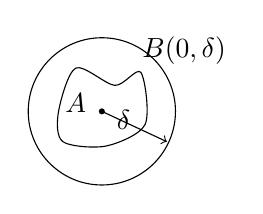
\begin{tikzpicture}[scale=.55]\draw (0,0) circle(1.7);\draw plot[smooth cycle] coordinates{(-1,0)(-.6,1)(.3,.6)(.9,.9)(1,-.3)(.1,-.8)(-.9,-.7)};\fill(0,0)circle(2pt);\draw[->](0,0)--(1.5,-.7);\node at(.5,-.2){$\delta$};\node at(-.6,.2){$A$};\node at(1.9,1.4){$B(0,\delta)$};\end{tikzpicture}\end{center}
% Pagina originale 16
\pagina{16}
\subsection*{Massimo e minimo}
$f:A\subset\R^n\to\R$. $M$ è massimo se $f(M)\ge f(x)$ per ogni $x\in A$; $m$ è minimo se $f(m)\le f(x)$ per ogni $x\in A$.
\subsection*{Insieme compatto}
$A\subset\R^n$ compatto $\iff A$ chiuso e limitato.
Osservazione: $\R^n$ e $\varnothing$ sono gli unici insiemi che sono sia aperti che chiusi. $\varnothing$ è compatto; $\R^n$ no, perché non è limitato.
\subsection*{Compattezza $\iff$ compattezza sequenziale}
$A\subset\R^n$ compatto se e solo se per ogni successione $(a_n)\subset A$ esistono indici $n_k\in\N$, $n_k<n_{k+1}$, tali che $a_{n_k}\to\bar x\in A$. Esempio di indici: $1,2,5,7,10,13,\ldots$.
\subsection*{4. Teorema di Weierstrass}
Ipotesi: $f:A\subset\R^n\to\R$, $A$ compatto, $f\in C^0(A)$. Tesi: $f$ ha minimo e massimo.
Dimostrazione, nel caso del minimo: $f(A)$ ha minimo $\iff\inf f(A)\in f(A)$.
Se $f\in C^0(A)$, $\inf f(A)\ne-\infty$ (appartiene a $\R$).
$\inf f(A)=\lambda\in\R$. Per ogni $n\in\N$ esiste $a_n\in A$ tale che $\lambda\le f(a_n)<\lambda+1/n$.
% Pagina originale 17
\pagina{17}
$\lambda\le f(a_n)\le\lambda+1/n$. Per $n\to+\infty$, gli estremi tendono a $\lambda$, quindi $f(a_n)\to\lambda=\inf f(A)$.
$A$ è compatto, dunque sequenzialmente compatto: esiste $(n_k)\subset\N$, $n_k<n_{k+1}$, con $a_{n_k}\to\bar x\in A$.
Per continuità $f(a_{n_k})\to f(\bar x)$. D'altra parte $f(a_n)\to\lambda\Rightarrow f(a_{n_k})\to\lambda=f(\bar x)$, e $\lim_{x\to\bar x}f(x)=f(\bar x)$.
\subsection*{5. Una funzione continua trasforma compatto in compatto}
Ipotesi: $f:A\subset\R^n\to\R$, $f\in C^0(A)$, $K\subset A$ compatto. Tesi: $f(K)$ compatto.
Dimostrazione: per ogni $(y_n)\subset f(K)$ dobbiamo trovare $n_k<n_{k+1}$ con $y_{n_k}\to\bar y\in f(K)$.
Per ogni $n\in\N$ esiste $x_n\in K$ tale che $f(x_n)=y_n$.
$(x_n)\subset K\Rightarrow\exists(n_k)\subset\N$, $n_k<n_{k+1}$, tale che $x_{n_k}\to\bar x\in K$.
$f(x_{n_k})=y_{n_k}\to f(\bar x)=\bar y$, e $f(\bar x)\in f(K)$.
% Pagina originale 18
\pagina{18}
\subsection*{$f^{-1}(B)$ aperto (chiuso) se $B$ aperto (chiuso)}
Ipotesi: $f:A\subset\R^n\to\R^m$, $f\in C^0(\operatorname{dom}f)$.
Tesi: per ogni $B\subset\R^m$ aperto, $f^{-1}(B)\subset A\subset\R^n$ aperto; per ogni $B\subset\R^m$ chiuso, $f^{-1}(B)\subset A\subset\R^n$ chiuso.
\nota{Le proprietà vanno intese nella topologia relativa di $A$; l'originale non precisa questo punto.}
\subsection*{Unioni e intersezioni tra insiemi aperti/chiusi}
1) Sia $(A_\alpha)_{\alpha\in I}\subset\R^n$ una famiglia di aperti. $\bigcup_{\alpha\in I}A_\alpha$ è aperto; $\bigcap_{\alpha\in I}A_\alpha$ è aperto se la famiglia è finita.
2) Sia $(A_\alpha)_{\alpha\in I}\subset\R^n$ una famiglia di chiusi. $\bigcup_{\alpha\in I}A_\alpha$ è chiuso se la famiglia è finita; $\bigcap_{\alpha\in I}A_\alpha$ è chiuso.
\nota{Nell'originale entrambe le condizioni di finitezza sono scritte con un'equivalenza: in generale sono condizioni sufficienti.}
\subsection*{Insieme convesso}
$A\subset\R^n$ si dice convesso se $\forall x,y\in A\ \forall\lambda\in[0,1]:\ (1-\lambda)x+\lambda y\in A$.
\begin{center}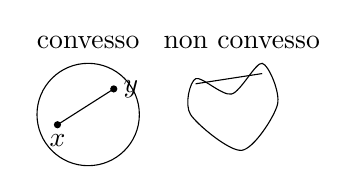
\begin{tikzpicture}[scale=.65]\draw(0,0)circle(1);\fill(-.6,-.2)circle(2pt);\fill(.5,.5)circle(2pt);\draw(-.6,-.2)--(.5,.5);\node[below] at(-.6,-.2){$x$};\node[right] at(.5,.5){$y$};\node at(0,1.4){convesso};\draw plot[smooth cycle] coordinates{(2,0)(2.1,.7)(2.8,.4)(3.4,1)(3.7,.2)(3,-.7)};\draw(2.1,.6)--(3.4,.8);\node at(3,1.4){non convesso};\end{tikzpicture}\end{center}
\subsection*{Insieme connesso per archi}
$A\subset\R^n$ connesso per archi se $\forall x,y\in A\ \exists\gamma:[a,b]\to\R^n$, $\gamma\in C^0([a,b])$, tale che $\gamma(a)=x$, $\gamma(b)=y$, $\gamma([a,b])\subset A$.
% Pagina originale 19
\pagina{19}
\subsection*{Convesso $\Rightarrow$ connesso per archi}
Esiste $\gamma:[0,1]\to\R^n$, $\gamma(t)=(1-t)x+ty$, con $\gamma(0)=x$, $\gamma(1)=y$, $\gamma([0,1])\subset A$.
\subsection*{6. Teorema degli zeri per $\R^n$}
Ipotesi: $f:A\subset\R^n\to\R$, $f\in C^0(A)$, $C\subset A$ connesso per archi, $x,y\in C$, $f(x)f(y)<0$.
Tesi: $\exists z\in C:\ f(z)=0$.
Dimostrazione: $C$ connesso per archi implica $\exists\gamma:[a,b]\to\R^n$ continua, $\gamma(a)=x$, $\gamma(b)=y$, $\gamma([a,b])\subset C$.
Considero $f\circ\gamma:[a,b]\to\R$, con $f(\gamma(a))=f(x)$, $f(\gamma(b))=f(y)$ e $f(\gamma(a))f(\gamma(b))<0$.
Esiste $c\in(a,b)$ tale che $f(\gamma(c))=0$ per il teorema degli zeri in $\R$. Quindi $z=\gamma(c)\in C$.
\subsection*{$f$ trasforma connessi in connessi}
$f:A\subset\R^n\to\R^m$, $f\in C^0(A)$: per ogni $C\subset A$ connesso per archi, $f(C)$ è connesso per archi.
% Pagina originale 20
\pagina{20}
\section*{Rapporto incrementale}
$f:A\subset\R^n\to\R^m$, $v$ versore.
\[\lim_{t\to0}\frac{f(x_0+tv)-f(x_0)}t=\ell\in\R^m.\]
$\ell$ è la derivata direzionale nella direzione $v$. Se $v$ è un componente della base canonica, $\ell$ è una derivata parziale.
\subsection*{Gradiente}
Per $f:A\subset\R^n\to\R$,
\[\nabla f(x_0)=\left(\frac{\partial f}{\partial x^1}(x_0),\frac{\partial f}{\partial x^2}(x_0),\ldots,\frac{\partial f}{\partial x^n}(x_0)\right).\]
\subsection*{Jacobiano e matrice jacobiana}
Per $f:A\subset\R^n\to\R^m$,
\[J_f(x_0)=\begin{pmatrix}\partial f^1/\partial x^1&\cdots&\partial f^1/\partial x^n\\\partial f^2/\partial x^1&\cdots&\partial f^2/\partial x^n\\\vdots&\ddots&\vdots\\\partial f^m/\partial x^1&\cdots&\partial f^m/\partial x^n\end{pmatrix}_{x_0}.\]
$\det J_f(x_0)$ è lo jacobiano (solo se $f:A\subset\R^n\to\R^n$).
\subsection*{Differenziabilità}
$f:A\subset\R^n\to\R^m$, $x_0\in\mathring A$. $f$ è differenziabile in $x_0$ se esiste una mappa lineare $L_{x_0}:\R^n\to\R^m$ tale che
\[\lim_{x\to x_0}\frac{f(x)-f(x_0)-L_{x_0}(x-x_0)}{|x-x_0|}=\bar0.\]
% Pagina originale 21
\pagina{21}
$f$ differenziabile in $x_0$ se e solo se per ogni $i=1,\ldots,m$,
\[\lim_{x\to x_0}\frac{f^i(x)-f^i(x_0)-L_{x_0}^i(x-x_0)}{|x-x_0|}=0.\]
\subsection*{Miglior approssimazione lineare}
$f$ differenziabile $\iff f$ ha miglior approssimazione lineare:
\[f(x)=f(x_0)+L_{x_0}(x-x_0)+o(|x-x_0|).\]
\subsection*{7. Differenziabile $\Rightarrow$ continua}
Ipotesi: $f:A\subset\R^n\to\R^m$, $x_0\in\mathring A$, $f$ differenziabile in $x_0$. Tesi: $f$ continua in $x_0$.
Dimostrazione: $x_0$ interno implica punto di accumulazione. $f$ continua in $x_0\iff\lim_{x\to x_0}f(x)=f(x_0)$.
$f(x)-f(x_0)=L_{x_0}(x-x_0)+o(|x-x_0|)$.
Per $x\to x_0$ entrambi gli addendi tendono a $0$, quindi $f(x)-f(x_0)\to0\Rightarrow f(x)\to f(x_0)$.
\subsection*{Cos'è la mappa lineare $L_{x_0}$}
$L_{x_0}(x-x_0)=A_{x_0}(x-x_0)$, prodotto righe per colonne, con $A_{x_0}\in M(m,n)$ e $(x-x_0)$ vettore colonna. Dimostriamo che $A_{x_0}=J_f(x_0)$.

% Pagina originale 22
\pagina{22}
\subsection*{8. Differenziabilità $\Rightarrow\exists J_f$ e $A_{x_0}=J_f(x_0)$}
Ipotesi: $f:A\subset\R^n\to\R^m$, $x_0\in\mathring A$, $f$ differenziabile. Tesi: esiste $J_f(x_0)$ e $L_{x_0}(x-x_0)=J_f(x_0)(x-x_0)$.
Dimostrazione: $f$ differenziabile implica $f^i$ differenziabile per ogni $i=1,\ldots,m$. Fissiamo $i\in\{1,\ldots,m\}$ e $j\in\{1,\ldots,n\}$:
\[\lim_{x\to x_0}\frac{f^i(x)-f^i(x_0)-L^i_{x_0}(x-x_0)}{|x-x_0|}=0,\quad\lim_{h\to0}\frac{f^i(x_0+h)-f^i(x_0)-L^i_{x_0}(h)}{|h|}=0.\]
Sia $h=te_j$, allora $|h|=|te_j|=|t||e_j|=|t|$:
\[\lim_{t\to0}\frac{f^i(x_0+te_j)-f^i(x_0)-L^i_{x_0}(te_j)}{|t|}=0.\]
\[\lim_{t\to0}\left|\frac{f^i(x_0+te_j)-f^i(x_0)-L^i_{x_0}(te_j)}{|t|}\right|=0
\iff\lim_{t\to0}\frac{|f^i(x_0+te_j)-f^i(x_0)-L^i_{x_0}(te_j)|}{|t|}=0.\]
Si può sostituire $|t|$ con $t$ dentro il valore assoluto, e togliere il valore assoluto:
\[\lim_{t\to0}\frac{f^i(x_0+te_j)-f^i(x_0)-L^i_{x_0}(te_j)}t=0.\]
Per linearità $L^i_{x_0}(te_j)=tL^i_{x_0}(e_j)$, dunque
\[\lim_{t\to0}\left[\frac{f^i(x_0+te_j)-f^i(x_0)}t-\frac{tL^i_{x_0}(e_j)}t\right]=0,
\quad\lim_{t\to0}\frac{f^i(x_0+te_j)-f^i(x_0)}t=L^i_{x_0}(e_j)=a^i_j.\]
Il limite a sinistra è $\frac{\partial f^i}{\partial x^j}(x_0)=a^i_j$, quindi $J_f(x_0)=A_{x_0}$.
% Pagina originale 23
\pagina{23}
\subsection*{9. Differenziabilità $\Rightarrow f$ ha tutte le derivate direzionali}
Ipotesi: $f:A\subset\R^n\to\R^m$, $x_0\in\mathring A$, $f$ differenziabile. Tesi: $f$ ha tutte le derivate direzionali e
\[\frac{\partial f}{\partial v}(x_0)=L_{x_0}(v)=J_f(x_0)v.\]
Dimostrazione: sia $v\in\R^n$ versore, $|v|=1$. $h=tv$ implica $|h|=|t||v|=|t|$;
\[\lim_{t\to0}\frac{f(x_0+tv)-f(x_0)-L_{x_0}(tv)}{|t|}=0,
\quad\lim_{t\to0}\frac{f(x_0+tv)-f(x_0)}t=L_{x_0}(v).\]
Quindi esiste $\frac{\partial f}{\partial v}(x_0)=L_{x_0}(v)=J_f(x_0)v$.
Osservazione: per $f:A\subset\R^n\to\R$, $J_f(x_0)=\nabla f(x_0)$, quindi
\[\frac{\partial f}{\partial v}(x_0)=\nabla f(x_0)\cdot v=\sum_{i=1}^n\frac{\partial f}{\partial x^i}(x_0)v^i.\]
\subsection*{Teorema del differenziale}
Ipotesi: $f:A\subset\R^n\to\R^m$, $x_0\in\mathring A$. Esiste un intorno $U$ di $x_0$ tale che per ogni $x\in U$ esistono le derivate $\frac{\partial f}{\partial x_i}(x)$, $i=1,\ldots,n$;
\[\frac{\partial f}{\partial x_i}:U\to\R^m,
\quad\frac{\partial f}{\partial x_i}(x)=\left(\frac{\partial f^1}{\partial x_i}(x),\ldots,\frac{\partial f^m}{\partial x_i}(x)\right),\]
con tutte le componenti continue in $x_0$. Tesi: $f$ è differenziabile in $x_0$.
% Pagina originale 24
\pagina{24}
\subsection*{Corollario}
Se $f$ ha derivate parziali e ogni derivata parziale è continua, allora $f$ è differenziabile.
\subsection*{Differenziale}
Miglior approssimazione lineare: $x\in\R^n\mapsto f(x_0)+J_f(x_0)(x-x_0)$.
Differenziale: $h\in\R^n\mapsto J_f(x_0)h$.
\subsection*{Derivate di funzioni composte}
$f:A\subset\R^n\to\R^m$, $g:B\subset\R^m\to\R^k$, $f(A)\subset B$, $x_0\in\mathring A$, $f(x_0)\in\mathring B$. Se $f$ è differenziabile in $x_0$ e $g$ in $f(x_0)$, allora $g\circ f$ è differenziabile in $x_0$ e
\[J_{g\circ f}(x_0)=J_g(f(x_0))J_f(x_0).\]
\subsection*{Corollario}
$\gamma:I\subset\R\to A\subset\R^n$, $f:A\to\R$. Se $t_0\in\mathring I$, $\gamma$ derivabile in $t_0$, $\gamma(t_0)\in\mathring A$ e $f$ differenziabile in $\gamma(t_0)$, allora $f\circ\gamma$ è derivabile in $t_0$ e
\[\frac{d}{dt}(f\circ\gamma)(t_0)=\nabla f(\gamma(t_0))\cdot\gamma'(t_0).\]
% Pagina originale 25
\pagina{25}
\subsection*{Curva di livello}
$f:A\subset\R^n\to\R$, $c\in\R$. $f^{-1}(\{c\})\subset A$ è la curva di livello $c$ di $f$. Se $c\notin\operatorname{Im}f$, allora $f^{-1}(\{c\})=\varnothing$.
Notazioni: $f^c=f^{-1}(({-\infty},c])$, $f_c=f^{-1}([c,+\infty))$.
\subsection*{10. Ortogonalità tra gradiente e tangente}
$f:A\subset\R^n\to\R$, $A=\mathring A$, $c\in\R$, $f^{-1}(\{c\})\ne\varnothing$. Esiste $\gamma:I\to A$ con $\gamma(I)\subset f^{-1}(\{c\})$. Sia $x_0\in f^{-1}(\{c\})\cap\gamma(I)$; $f$ differenziabile in $x_0$, $\nabla f(x_0)\ne\bar0$. Sia $t_0\in I$ con $\gamma(t_0)=x_0$. Allora $\nabla f(x_0)\perp\gamma'(t_0)$.
Dimostrazione: $(f\circ\gamma)(t)=c$ per ogni $t\in I$, quindi $\frac d{dt}(f\circ\gamma)(t_0)=0=\nabla f(x_0)\cdot\gamma'(t_0)$.
\begin{center}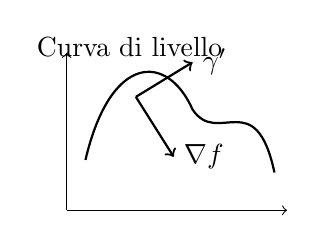
\begin{tikzpicture}[scale=.8]
\draw[->] (0,0)--(3.5,0);\draw[->] (0,0)--(0,2.5);
\draw[thick] (.3,.8) .. controls (.7,2.5) and (1.6,2.5) .. (2,1.6) .. controls (2.4,1) and (3,2) .. (3.3,.6);
\draw[->,thick] (1.1,1.8)--(2,2.35) node[right] {$\gamma'$};
\draw[->,thick] (1.1,1.8)--(1.7,.85) node[right] {$\nabla f$};
\node at (1,2.6) {Curva di livello};
\end{tikzpicture}\end{center}
\subsection*{11. Direzione di massima crescita}
$f:A\subset\R^n\to\R$, $x_0\in\mathring A$, $f$ differenziabile in $x_0$, $\nabla f(x_0)\ne\bar0$ per normalizzare. $\nabla f(x_0)/|\nabla f(x_0)|$ è la direzione di massima crescita per $f$.
% Pagina originale 26
\pagina{26}
Dimostrazione:
\[\frac{\partial f}{\partial v}(x_0)=\nabla f(x_0)\cdot v=|\nabla f(x_0)||v|\cos\theta.\]
Ha il massimo per $\cos\theta=1$, ossia $\theta=2\pi k$: $v\parallel\nabla f$, quindi $v=\nabla f(x_0)/|\nabla f(x_0)|$.
\subsection*{Massimo/minimo locale di una funzione}
$f:A\subset\R^n\to\R$, $x_0\in A$. $x_0$ minimo locale se esiste un intorno $U$ di $x_0$ con $f(x)\ge f(x_0)$ per ogni $x\in U\cap A$, cioè $f(x)-f(x_0)\ge0$. $x_0$ massimo locale se esiste $U$ con $f(x)\le f(x_0)$ per ogni $x\in U\cap A$, dunque $f(x_0)-f(x)\ge0$.
\subsection*{12. Teorema di Fermat}
$f:A\subset\R^n\to\R$, $x_0\in\mathring A$, $f$ derivabile in $x_0$. $x_0$ punto estremale implica $\nabla f(x_0)=\bar0$.
Dimostrazione: prendo $n$ rette del tipo $r_i:t\in\R\mapsto x_0+te_i$, $i=1,\ldots,n$. Sia $\varepsilon>0$ con $B(x_0,\varepsilon)\subset A$. Esiste $\delta>0$ con $r_i(t)\in B(x_0,\varepsilon)$ per ogni $t\in(-\delta,\delta)$ e ogni $i$. $x_0$ estremo locale in $f$ implica che $t=0$ è estremo locale in $f\circ r_i$.
\begin{center}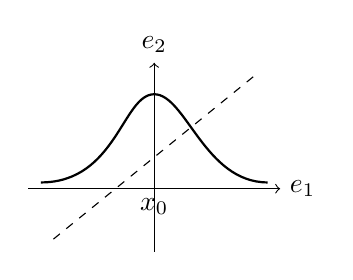
\begin{tikzpicture}[scale=.8]
\draw[->] (-2,0)--(2,0) node[right] {$e_1$};\draw[->] (0,-1)--(0,2) node[above] {$e_2$};
\draw[thick] (-1.8,.1).. controls(-.6,.1) and(-.5,1.5)..(0,1.5)..controls(.5,1.5) and(.8,.1)..(1.8,.1);
\draw[dashed] (-1.6,-.8)--(1.6,1.8);\node[below] at(0,0){$x_0$};
\end{tikzpicture}\end{center}
% Pagina originale 27
\pagina{27}
\[\left(f\circ r_i|_{(-\delta,\delta)}\right)'(0)=0=\nabla f(r_i(0))\cdot r_i'(0).\]
\[\left(f\circ r_i|_{(-\delta,\delta)}\right)'(0)=\lim_{h\to0}\frac{f(r_i(h))-f(r_i(0))}{h}=\frac{\partial f}{\partial e_i}(x_0)=0,\quad i=1,\ldots,n.\]
\subsection*{Punto critico singolare}
$x_0$ è punto critico per $f$ se $J_f(x_0)=\bar0$ (più precisamente quando $J_f$ è singolare).
\subsection*{13. Teorema di Lagrange}
$f:A\subset\R^n\to\R$, $A$ convesso, $f$ differenziabile, $A=\mathring A$. $S(x,y):\lambda\in[0,1]\mapsto(1-\lambda)x+\lambda y$. Per ogni $x,y\in A$ esiste $\xi\in S(x,y)\subset A$ tale che
\[f(y)-f(x)=\nabla f(\xi)\cdot(y-x).\]
Dimostrazione: $f\circ S:[0,1]\to\R$ è derivabile poiché $f$ è differenziabile e $S$ derivabile. $S'(\lambda)=-x+y=y-x$ per ogni $\lambda\in[0,1]$. Dal teorema di Lagrange esiste $\theta\in(0,1)$ con
\[(f\circ S)(1)-(f\circ S)(0)=(f\circ S)'(\theta)(1-0).\]
Quindi $f(y)-f(x)=\nabla f(S(\theta))\cdot S'(\theta)=\nabla f(S(\theta))\cdot(y-x)$; $\xi=S(\theta)$.
\subsection*{Localmente lipschitziana}
Una $f$ è localmente lipschitziana se esiste $L>0$ tale che $|f(y)-f(x)|\le L|y-x|$.
% Pagina originale 28
\pagina{28}
\subsection*{Derivata seconda direzionale}
$f:A\subset\R^n\to\R^m$, $x_0\in\mathring A$, $|v|=|w|=1$. Esiste $\delta>0$ tale che per ogni $x\in B(x_0,\delta)\subset A$ esiste $\partial f/\partial v(x)$. Se esiste
\[\lim_{t\to0}\frac{\frac{\partial f}{\partial v}(x_0+tw)-\frac{\partial f}{\partial v}(x_0)}t=\ell\in\R^m,\]
$f$ ha derivata direzionale di ordine 2 rispetto ai versori $v,w$.
\subsection*{Derivata seconda parziale}
Siano $i,j\in\{1,\ldots,n\}$. Se esiste $\frac{\partial}{\partial e_j}(\frac{\partial f}{\partial e_i})(x_0)=\frac{\partial^2f}{\partial e_j\partial e_i}(x_0)$, $f$ è derivabile due volte parzialmente rispetto a $e_i,e_j$.
\subsection*{Hessiano}
$f:A\subset\R^n\to\R$, $x_0\in\mathring A$; $f$ ha tutte le derivate parziali del secondo ordine in $x_0$:
\[\operatorname{Hess}_f(x_0)=\begin{pmatrix}f_{x_1x_1}&f_{x_1x_2}&\cdots&f_{x_1x_n}\\f_{x_2x_1}&f_{x_2x_2}&\cdots&f_{x_2x_n}\\\vdots&\vdots&\ddots&\vdots\\f_{x_nx_1}&f_{x_nx_2}&\cdots&f_{x_nx_n}\end{pmatrix}_{x_0}.\]
\subsection*{Teorema di Schwartz}
Siano $f_{x_ix_j}$ e $f_{x_jx_i}$ definite in un intorno di $x_0$: esiste $U$ intorno di $x_0$ con $f_{x_ix_j}(x),f_{x_jx_i}(x)\in\R$ per ogni $x\in U$. Se sono continue in $x_0$, allora $f_{x_ix_j}(x_0)=f_{x_jx_i}(x_0)$.
% Pagina originale 29
\pagina{29}
\subsection*{Corollario}
$f\in C^2(A,\R)\Rightarrow f_{x_ix_j}=f_{x_jx_i}$ per ogni $i,j\in\{1,\ldots,n\}$.
\subsection*{Classi $C$}
\[C^0(A,\R^m)=\{f:A\to\R^m:\ f^j\text{ continua per ogni }j=1,\ldots,m\},\]
\[C^n(A,\R^m)=\{f:A\to\R^m:\ f^j\text{ ha tutte le derivate parziali di ordine }n\text{ continue},\ j=1,\ldots,m\}.\]
\[C^\infty(A)\subsetneq C^{k+1}(A)\subsetneq C^k(A)\subsetneq C^{k-1}(A)\subsetneq C^0(A).\]
Osservazione: se $f\in C^2(A)$, $\operatorname{Hess}_f$ è simmetrica.
\subsection*{Forma quadratica}
\[q(a,b,c)=h_1a^2+h_2ab+h_3ac+h_4b^2+h_5ba+h_6bc+h_7c^2+h_8ca+h_9cb.\]
\[A=\begin{pmatrix}h_1&h_2&h_3\\h_5&h_4&h_6\\h_8&h_9&h_7\end{pmatrix},\qquad q(a,b,c)=(a,b,c)A\begin{pmatrix}a\\b\\c\end{pmatrix}.\]
Una forma quadratica è un polinomio omogeneo di grado 2. $q(\lambda v)=\lambda^2q(v)$, $q(v)=v\cdot Av$.
% Pagina originale 30
\pagina{30}
\subsection*{Segno di una forma quadratica}
Sia $q:\R^n\to\R$ una forma quadratica. $q$ è definita positiva se $q(v)>0$ per ogni $v\in\R^n\setminus\{\bar0\}$; è semidefinita positiva se $q(v)\ge0$ per ogni $v\in\R^n$. Se esistono $v_1,v_2\in\R^n\setminus\{\bar0\}$ con $q(v_1)>0$ e $q(v_2)<0$, $q$ è indefinita.
Osservazione: $\partial B(\bar0,1)=\{x\in\R^n:|x|=1\}$ è compatto, quindi $q$ vi ha minimo e massimo. Per $v\ne\bar0$, $v/|v|\in S^{n-1}(1)=\partial B(\bar0,1)$,
\[q(v)=q\left(|v|\frac v{|v|}\right)=|v|^2q\left(\frac v{|v|}\right).\]
Poiché $|v|^2>0$, il segno dipende esclusivamente da $q(v/|v|)$. Se il minimo di $q$ sulla sfera è positivo, $q$ è definita positiva; se il massimo è negativo, è definita negativa.
\subsection*{Scorciatoia per il segno di una forma quadratica}
Sia $q:\R^2\to\R$, $q(x,y)=ax^2+bxy+cy^2$. Dividiamo per $x$ se $x\ne0$, per $y$ se $y\ne0$. Supponiamo $y\ne0$:
\[q(x,y)=y^2\left(a\left(\frac xy\right)^2+b\frac xy+c\right)=y^2(at^2+bt+c),\qquad t=\frac xy.\]
Se $at^2+bt+c>0$, $q$ è definita positiva; se $\ge0$, semidefinita positiva; se $\le0$, semidefinita negativa; se $<0$, definita negativa.
% Pagina originale 31
\pagina{31}
\[A_q=\begin{pmatrix}a&b/2\\b/2&c\end{pmatrix}.\]
Se $a>0$ e $\Delta<0$, allora $q>0$ per ogni vettore non nullo.
\[\det A_q=ac-\frac{b^2}4=-\frac14(b^2-4ac)=-\frac14\Delta.\]
Se $\det A_q>0$, $\Delta<0$. In definitiva:
\[\begin{array}{c|c|l}\det A_q&a&\text{segno}\\\hline>0&>0&\text{positiva}\\=0&>0&\text{semipositiva}\\=0&<0&\text{seminegativa}\\>0&<0&\text{negativa}\\<0&&\text{indefinita}\end{array}\]
\subsection*{Forma lineare o forma differenziale}
La funzione $x\in A\mapsto\omega(x)\in\mathcal L(\R^n,\R)$, spazio delle applicazioni lineari da $\R^n$ a $\R$, dove $\omega(x)(h)=\sum_{i=1}^n a_i(x)h^i$, è una forma lineare di coefficienti $a_i$.
\subsection*{14. Differenziabilità in $x_0$ due volte}
$f$ è differenziabile due volte in $x_0$ se: (1) $f$ è differenziabile; (2)
\[\lim_{h\to0}\frac{df(x_0+h)-df(x_0)-L_{x_0}(h)}{|h|}=0.\]
Sia $f:A\to\R$ differenziabile due volte in $x_0\in\mathring A$. Allora
\[f(x)=f(x_0)+\nabla f(x_0)\cdot(x-x_0)+\frac12\bigl(\operatorname{Hess}_f(x_0)(x-x_0)\bigr)\cdot(x-x_0)+o(|x-x_0|^2).\]
% Pagina originale 32
\pagina{32}
Quindi, per $x\to x_0$,
\[\frac{f(x)-f(x_0)-\nabla f(x_0)\cdot(x-x_0)-\frac12\bigl(\operatorname{Hess}_f(x_0)(x-x_0)\bigr)\cdot(x-x_0)}{|x-x_0|^2}\to0.\]
Dimostrazione: $x_0\in\mathring A\iff\exists\delta>0:B(x_0,\delta)\subset A$. Prendo $h$ con $|h|<\delta$. Consideriamo $v=h/|h|$ e $\gamma:t\in[0,|h|]\mapsto x_0+tv$, cosicché $\gamma(0)=x_0$, $\gamma(|h|)=x_0+h$.
$g=f\circ\gamma$ è derivabile (entrambe le funzioni sono differenziabili) su $[0,|h|]$:
\[g'(t)=\nabla f(\gamma(t))\cdot\gamma'(t)=\nabla f(\gamma(t))\cdot v.\]
$f\in C^2(U)$, $U=B(x_0,\delta)$, implica $g$ derivabile due volte:
\[g''(t)=\bigl(J_{\nabla f}(\gamma(t))\gamma'(t)\bigr)\cdot v=\bigl(\operatorname{Hess}_f(\gamma(t))v\bigr)\cdot v.\]
\[g(t)=g(0)+g'(0)t+\frac12g''(0)t^2+o(t^2).\]
Per $t=|h|$,
\[g(|h|)=g(0)+g'(0)|h|+\frac12g''(0)|h|^2+o(|h|^2),\]
\[f(x_0+h)=f(x_0)+\nabla f(x_0)\cdot\frac h{|h|}|h|+\frac12\left(\operatorname{Hess}_f(x_0)\frac h{|h|}\right)\cdot\frac h{|h|}|h|^2+o(|h|^2).\]
\subsection*{Formula di Taylor di ordine 2 per funzioni a più variabili}
\begin{align*}
f(x,y)={}&f(x_0,y_0)+f_x(x_0,y_0)(x-x_0)+f_y(x_0,y_0)(y-y_0)\\
&+\frac1{2!}\bigl[f_{xx}(x_0,y_0)(x-x_0)^2+f_{xy}(x_0,y_0)(x-x_0)(y-y_0)\\
&\hspace{22mm}+f_{yy}(x_0,y_0)(y-y_0)^2\bigr]+o((x-x_0)^2+(y-y_0)^2).
\end{align*}
\nota{Nell'originale il termine misto è scritto senza il fattore 2; è stato mantenuto.}
% Pagina originale 33
\pagina{33}
\subsection*{15. Condizione sufficiente perché un punto critico sia di estremo locale}
$f:A\subset\R^n\to\R$, $x_0\in\mathring A$, $f\in C^2(U)$, $x_0$ stazionario ($\nabla f(x_0)=\bar0$). Se la forma quadratica $h\in\R^n\mapsto(\operatorname{Hess}_f(x_0)h)\cdot h$ è: (1) definita positivamente, $x_0$ minimo locale forte; (2) definita negativamente, $x_0$ massimo locale forte; (3) indefinita, $x_0$ non è estremale (punto di sella).
Dimostrazione di (1), (2):
\[f(x)-f(x_0)=\frac12\bigl(H_f(x_0)(x-x_0)\bigr)\cdot(x-x_0)+o(|x-x_0|^2).\]
Suppongo $x\ne x_0$:
\[f(x)-f(x_0)=|x-x_0|^2\left[\frac12\left(H_f(x_0)\frac{x-x_0}{|x-x_0|}\right)\cdot\frac{x-x_0}{|x-x_0|}+\frac{o(|x-x_0|^2)}{|x-x_0|^2}\right].\]
Se $H_f(x_0)$ è definita positivamente,
\[f(x)-f(x_0)\ge|x-x_0|^2\left[\frac12\min_{v\in S^{n-1}(1)}(H_f(x_0)v)\cdot v+\frac{o(|x-x_0|^2)}{|x-x_0|^2}\right].\]
Se è definita negativamente,
\[f(x)-f(x_0)\le|x-x_0|^2\left[\frac12\max_{v\in S^{n-1}(1)}(H_f(x_0)v)\cdot v+\frac{o(|x-x_0|^2)}{|x-x_0|^2}\right].\]
Per $x\to x_0$, nel primo caso la parentesi tende a $\frac12\lambda_1(x_0)+0>0$. Per il teorema della permanenza del segno esiste un intorno $V$ di $x_0$ tale che
\[\frac12\lambda_1(x_0)+\frac{o(|x-x_0|^2)}{|x-x_0|^2}>0\quad\forall x\in V\subset A.\]

% Pagina originale 34
\pagina{34}
Se $x\to x_0$:
\[\tfrac12\max H_f(x_0)vv+\frac{o(|x-x_0|^2)}{|x-x_0|^2}\longrightarrow\tfrac12\lambda_n(x_0)+0<0.\]
Per il teorema della permanenza del segno esiste $V\in\mathcal I(x_0)$ tale che
\[\tfrac12\lambda_n(x_0)+\frac{o(|x-x_0|^2)}{|x-x_0|^2}<0\qquad\forall x\in V\subset A.\]
Dimostrazione 3): esistono $v_1,v_2\in\R^n\setminus\{\bar0\}$ tali che $H_f(x_0)v_1v_1>0$, $H_f(x_0)v_2v_2<0$. Considero $\lambda v_1$, con $\lambda\to0$: $\lambda^2H_f(x_0)v_1v_1>0$. Considero $\lambda v_2$, con $\lambda\to0$: $\lambda^2H_f(x_0)v_2v_2<0$.
\[f(x_0+\lambda v_1)-f(x_0)>0,\qquad f(x_0+\lambda v_2)-f(x_0)<0\quad\text{se }\lambda\sim0.\]
Quindi $x_0$ non è né di massimo né di minimo.
\subsection*{Condizione necessaria perché un punto critico sia di estremo locale}
$f:A\subset\R^n\to\R$, $x_0\in A^\circ$, $f\in C^2(V)$ con $V\in\mathcal I(x_0)$, $x_0$ stazionario ($\nabla f(x_0)=\bar0$). Allora:
\begin{itemize}
\item Se $x_0$ è massimo locale, $v\in\R^n\mapsto H_f(x_0)vv$ è semidefinita negativamente.
\item Se $x_0$ è minimo locale, $v\in\R^n\mapsto H_f(x_0)vv$ è semidefinita positivamente.
\end{itemize}
% Pagina originale 35
\pagina{35}
\section*{Integrale di Riemann a più variabili}
$\int_A f(x,y)\,dx\,dy$ rappresenta il volume del cilindroide. $A=[a,b]\times[c,d]$.
\subsection*{Suddivisione}
$D$ si definisce suddivisione di $A$ se $D=D_1\times D_2$ con $D_1\in\mathcal D([a,b])$ e $D_2\in\mathcal D([c,d])$.
\[Q_{ij}=[s_i,s_{i+1}]\times[t_j,t_{j+1}].\]
\subsection*{Somma inferiore/superiore}
\[s(f,D)=\sum_{i=0}^{n-1}\sum_{j=0}^{m-1}m_{ij}(s_{i+1}-s_i)(t_{j+1}-t_j),\]
\[S(f,D)=\sum_{i=0}^{n-1}\sum_{j=0}^{m-1}M_{ij}(s_{i+1}-s_i)(t_{j+1}-t_j).\]
Proprietà: $\forall D_1,D_2\in\mathcal D(A)$, $s(f,D_1)\le S(f,D_2)$.
\subsection*{Funzione integrabile}
$f:A\subset\R^2\to\R$, $Q\subset A$, $Q$ rettangolo; $f|_Q$ limitata.
% Pagina originale 36
\pagina{36}
$f$ è integrabile (secondo Riemann) in $Q$ se $\inf B=\sup A$, con
\[B:=\{S(f,D):D\in\mathcal D(Q)\},\qquad A:=\{s(f,D):D\in\mathcal D(Q)\}.\]
\[\int_Qf(x,y)\,dx\,dy=\int_a^b\int_c^d f(x,y)\,dx\,dy:=\inf B=\sup A.\]
\subsection*{Integrale doppio di funzioni costanti}
\[\int_Q K\,dx\,dy=\int_a^b\int_c^d K\,dx\,dy=K(b-a)(d-c),\qquad Q=[a,b]\times[c,d].\]
\subsection*{Continuità implica integrabilità}
Se $f\in C^0(A)$, $Q\subset A$, allora $f$ è integrabile in $Q$.
\subsection*{Caratterizzazione dell'integrabilità di una funzione definita su un rettangolo}
\[f\in\mathcal R(Q)\iff\forall\varepsilon>0\ \exists D\in\mathcal D(Q):S(f,D)-s(f,D)<\varepsilon.\]
\subsection*{Formula di riduzione}
$f\in\mathcal R(Q)$ (quindi limitata).
1) Se per ogni $x\in[a,b]$, $\int_c^d f(x,y)\,dy$ è integrabile, allora $x\in[a,b]\mapsto\int_c^d f(x,y)\,dy$ è integrabile e
\[\int_Qf=\int_a^b\int_c^d f\,dy\,dx.\]
% Pagina originale 37
\pagina{37}
2) Se per ogni $y\in[c,d]$, $\int_a^b f(x,y)\,dx$ è integrabile, allora $y\in[c,d]\mapsto\int_a^b f(x,y)\,dx$ è integrabile e
\[\int_Qf=\int_c^d\int_a^b f(x,y)\,dx\,dy.\]
\subsection*{Scambio dell'ordine di integrazione (o di inversione)}
\[\int_a^b\int_c^d f(x,y)\,dy\,dx=\int_c^d\int_a^b f(x,y)\,dx\,dy.\]
\subsection*{Funzioni a variabili separabili}
$f(x,y)$ si dice a variabili separabili se esistono $g:[a,b]\to\R$, $h:[c,d]\to\R$ tali che $f(x,y)=g(x)h(y)$.
\subsection*{16. Trasformazione di funzioni a variabili separabili}
Se $f$ è a variabili separabili con $f(x,y)=g(x)h(y)$, $f:Q\to\R$, $g\in C^0([a,b])$, $h\in C^0([c,d])$, allora $f\in C^0(Q)$ e
\[\int_c^d\int_a^b f=\int_a^b g(x)\,dx\cdot\int_c^d h(y)\,dy.\]
Dimostrazione:
\begin{align*}
\int_c^d\int_a^b f(x,y)\,dx\,dy&=\int_c^d\int_a^b g(x)h(y)\,dx\,dy\\
&=\int_c^d\left(h(y)\int_a^b g(x)\,dx\right)dy\\
&=\int_a^b g(x)\,dx\cdot\int_c^d h(y)\,dy.
\end{align*}
% Pagina originale 38
\pagina{38}
\subsection*{Integrabilità in $\Omega\subset R$, rettangolo}
$f$ è integrabile in $\Omega$ se, per ogni rettangolo $R$ tale che $\Omega\subset R$, la funzione
\[\widetilde f(x,y):=\begin{cases}f(x,y)&(x,y)\in\Omega,\\0&\text{altrimenti }(R\setminus\Omega),\end{cases}\qquad\widetilde f:R\to\R\]
è integrabile. Si pone
\[\int_\Omega f:=\int_\Omega\widetilde f+\int_{R\setminus\Omega}\widetilde f=\int_R\widetilde f.\]
L'integrazione è indipendente da $R$.
\subsection*{Insieme misurabile con misura zero}
$\Gamma\subset\R^2$ è misurabile di misura zero se
\[\forall\varepsilon>0\ \exists(R_i)_{i\in\{1,\ldots,n\}}:\Gamma\subset\bigcup_{i=1}^nR_i,\qquad\sum_{i=1}^n|R_i|<\varepsilon.\]
\subsection*{Insieme trascurabile}
$\Gamma$ è trascurabile se $|\Gamma|=0$. Ogni segmento è trascurabile. Ogni insieme finito di punti è trascurabile.
\subsection*{17. Il grafico di una funzione è trascurabile}
Ipotesi: $h:[a,b]\to\R$, $h\in\mathcal R([a,b])$. $G_h$ grafico della funzione.
% Pagina originale 39
\pagina{39}
Tesi: $G_h$ è trascurabile. Dimostrazione: $G_h$ è trascurabile se per ogni $\varepsilon>0$ esistono $\{R_i\}_{i=1}^n$ tali che $G_h\subset\bigcup_{i=1}^nR_i$ e $\sum_i|R_i|<\varepsilon$. $h$ è integrabile, quindi
\[\forall\varepsilon>0\ \exists D\in\mathcal D([a,b]):S(h,D)-s(h,D)<\varepsilon.\]
\[\sum_{i=1}^nM_i(t_i-t_{i-1})-m_i(t_i-t_{i-1})<\varepsilon
\implies\sum_{i=1}^n(M_i-m_i)(t_i-t_{i-1})<\varepsilon.\]
\subsection*{18. $\Omega$ misurabile se e solo se $\partial\Omega$ trascurabile}
Dimostrazione: $\Omega$ misurabile se e solo se $\mathbf1_\Omega$ è integrabile per ogni $R\supset\Omega$.
\[\forall\varepsilon>0\ \exists D\in\mathcal D(Q):S(\mathbf1_\Omega,D)-s(\mathbf1_\Omega,D)<\varepsilon.\]
\[S(\mathbf1_\Omega,D)-s(\mathbf1_\Omega,D)=\sum_{ij}(M_{ij}-m_{ij})|Q_{ij}|<\varepsilon.\]
Il fattore $M_{ij}-m_{ij}$ è $1$ solo nella frontiera.
\subsection*{Caratteristica di $\Omega$}
$\mathbf1_\Omega$ è la caratteristica di $\Omega$, $\mathbf1_\Omega:\R^2\to\R$:
\[\mathbf1_\Omega(x,y)=\begin{cases}1&(x,y)\in\Omega,\\0&\text{altrimenti}.\end{cases}\]
\[\int_\Omega1=\int_R\mathbf1_\Omega\quad\forall R\supset\Omega,\qquad\int_R\mathbf1_\Omega=|\Omega|\quad\text{(misura di }\Omega\text{)}.\]
% Pagina originale 40
\pagina{40}
Proprietà: se $(\Omega_i)_{i\in\{1,\ldots,n\}}$ sono misurabili, allora $\bigcup_{i=1}^n\Omega_i$ e $\bigcap_{i=1}^n\Omega_i$ sono misurabili. Osservazione: $\varnothing$ non è misurabile [come scritto nell'originale].
\[|\Omega_1|+|\Omega_2|=|\Omega_1\cup\Omega_2|+|\Omega_1\cap\Omega_2|.\]
Se $\Omega$ è trascurabile, ogni $\Omega'\subset\Omega$ è trascurabile. Per ogni $\Omega$ misurabile:
\[|\Omega|\inf_{x\in\Omega}f(x)\le\int_\Omega f\le\sup_{x\in\Omega}f(x)\,|\Omega|.\]
\subsection*{Media integrale}
\[M=\frac1{|\Omega|}\int_\Omega f\quad\text{se }|\Omega|\ne0,\qquad M=0\quad\text{se }|\Omega|=0.\]
Se $f\in\mathcal R(\Omega)$ e $\Omega$ è connesso per archi, allora esiste $\bar x\in\Omega$ tale che $f(\bar x)=\frac{\int_\Omega f}{|\Omega|}$.
Proprietà: $f\in\mathcal R(\Omega)$, $f\ge0$ (rispettivamente $\le0$) implica $\int_\Omega f\ge0$ (rispettivamente $\le0$).
\subsection*{Linearità dell'integrale}
\[\int_\Omega(\alpha f+\beta g)=\alpha\int_\Omega f+\beta\int_\Omega g.\]
Se $\Omega\subset\R^2$ misurabile, $\Omega_1,\Omega_2\subset\Omega$ misurabili, $\Omega_1\cup\Omega_2=\Omega$, $|\Omega_1\cap\Omega_2|=0$, $f\in\mathcal R(\Omega)$, allora $f\in\mathcal R(\Omega_1)\cap\mathcal R(\Omega_2)$ e
\[\int_\Omega f=\int_{\Omega_1}f+\int_{\Omega_2}f.\]
% Pagina originale 41
\pagina{41}
\subsection*{$\Gamma$ trascurabile contenuto in $\Omega$}
$f:\Omega\to\R$, $\Omega$ misurabile, $f\in\mathcal R(\Omega\setminus\Gamma)$: allora $f\in\mathcal R(\Omega)$ e $\int_\Omega f=\int_{\Omega\setminus\Gamma}f$.
\subsection*{Corollario}
$f\in C^0(\Omega\setminus\Gamma)$ e limitata in $\Omega$ implica $f\in\mathcal R(\Omega)$ e $\int_{\mathring\Omega}f=\int_\Omega f$, con $\mathring\Omega=\bar\Omega\setminus\partial\Omega$, perché
\[\int_{\mathring\Omega}f=\int_{\bar\Omega}f-\underbrace{\int_{\partial\Omega}f}_{0}=\int_{\bar\Omega}f.\]
\subsection*{Funzioni generalmente continue}
Se $f\in C^0(\Omega\setminus\Gamma)$, $f$ è generalmente continua in tutto $\Omega$.
\subsection*{Generalmente continua e limitata}
$f$ generalmente continua e limitata implica $f\in\mathcal R(\Omega)$.
\[\int_R\mathbf1_\Omega\in\R\iff f:\Omega\to\R\text{ generalmente continua in }\Omega.\]
\subsection*{Domini normali (o semplici)}
$\Omega\subset\R^2$ si dice normale rispetto all'asse $x$ se esistono $g,h\in C^0([a,b])$, $g,h:[a,b]\to\R$, $g\le h$, tali che
\[\Omega=\{(x,y)\in\R^2:x\in[a,b],\ g(x)\le y\le h(x)\}.\]
$\Omega$ è normale rispetto all'asse $y$ se esistono $g,h\in C^0([a,b])$, $g,h:[a,b]\to\R$, $g\le h$, tali che
\[\Omega=\{(x,y)\in\R^2:y\in[a,b],\ g(y)\le x\le h(y)\}.\]
% Pagina originale 42
\pagina{42}
Esempi: domini compresi fra i grafici $g(x),h(x)$ e fra $g(y),h(y)$.
\subsection*{19. Dominio $\Omega$ normale implica $\Omega$ misurabile}
Dimostrazione: $\partial\Omega$ è unione di quattro insiemi trascurabili:
\[\partial\Omega=S_1\cup S_2\cup G_h\cup G_g,\qquad|\partial\Omega|=0\iff\Omega\text{ misurabile}.\]
\[|\partial\Omega|=|S_1|+|S_2|+|G_h|+|G_g|-|S_1\cap S_2\cap G_h\cap G_g|=0+0+0+0-|\varnothing|=0.\]
\subsection*{20. Formula di riduzione su domini normali}
$\Omega\subset\R^2$ normale rispetto all'asse $x$:
\[\Omega=\{(x,y)\in\R^2:x\in[a,b],\ g(x)\le y\le h(x)\}.\]
Se $f\in C^0(\Omega)$, quindi $f\in\mathcal R(\Omega)$ e $f$ limitata,
\[\int_\Omega f=\int_a^b\int_{g(x)}^{h(x)}f(x,y)\,dy\,dx.\]
Dimostrazione: prendo un rettangolo $R$ tale che $\Omega\subset R$ e definisco
\[\widetilde f:=\begin{cases}f(x,y)&(x,y)\in\Omega,\\0&\text{altrimenti}.\end{cases}\]
$\widetilde f$ è integrabile perché limitata e generalmente continua. $R=[a,b]\times[c,d]$ con $d>\max h$, $c<\min g$.
\[\int_\Omega f=\int_R\widetilde f=\int_a^b\int_c^d\widetilde f=\int_a^b\int_{g(x)}^{h(x)}\widetilde f,\]
perché
\[\int_c^d\widetilde f=\underbrace{\int_c^{g(x)}\widetilde f}_{0}+\int_{g(x)}^{h(x)}\widetilde f+\underbrace{\int_{h(x)}^d\widetilde f}_{0}.\]
% Pagina originale 43
\pagina{43}
\subsection*{Formula del cambio di variabile}
Sia $\chi:A\subset\R^2\to B\subset\R^2$, $\chi=(\chi_1,\chi_2)$. $J_\chi(u,v)$ si indica come $\frac{\partial(x,y)}{\partial(u,v)}$. $\chi$ deve avere matrice jacobiana, quindi $\chi\in C^1(A)$, essere biiettiva, ed esiste $\Gamma$ trascurabile tale che per ogni $(u,v)\in A\setminus\Gamma$, $\det J\ne0$.
\subsection*{$\chi$ trasforma misurabili in misurabili}
Ipotesi: $f:\Omega\subset B\to\R$, $f$ limitata e $f\in C^0(\Omega)$; $\chi:\Omega'\subset A\to B$, $\chi\in C^1(\Omega')$, biiettiva e $\Gamma$ trascurabile tale che $|J|\ne0$ fuori da $\Gamma$. $\Omega=\chi(\Omega')$. $\Omega$ misurabile implica $\Omega'$ misurabile.
Tesi:
\[\int_\Omega f(x,y)\,dx\,dy=\int_{\Omega'}f\circ\chi(u,v)|J_\chi(u,v)|\,du\,dv.\]
\subsection*{Scelta di $\chi$ partendo da $\chi^{-1}$}
\[\begin{cases}u=\psi_1(x,y),\\v=\psi_2(x,y),\end{cases}\qquad\psi=\chi^{-1}.\]
$\psi\circ\chi=i_A$, identità di $A$.
\[J_{\psi\circ\chi}=J_\psi(\chi(u,v))J_\chi(u,v)=I.\]
Per il teorema di Binet, $|J_{\psi\circ\chi}|=|J_\psi(\chi(u,v))|\,|J_\chi(u,v)|$, quindi
\[|J_\chi(u,v)|=\frac1{|J_\psi(\psi(u,v))|}.\]
% Pagina originale 44
\pagina{44}
\subsection*{21. $\displaystyle\int_{-\infty}^{+\infty}e^{-x^2}\,dx=\sqrt\pi$}
\[\int_{-\infty}^{+\infty}e^{-x^2}\,dx=2\int_0^{+\infty}e^{-x^2}\,dx.\]
Calcolo
\[\left[\int_0^{+\infty}e^{-x^2}\,dx\right]^2=\int_0^{+\infty}e^{-x^2}\,dx\int_0^{+\infty}e^{-y^2}\,dy=\lim_{\omega\to+\infty}\int_{[0,\omega]\times[0,\omega]}e^{-(x^2+y^2)}\,dx\,dy.\]
\[\int_{D(0,\omega)}e^{-x^2-y^2}\le\int_{Q(\omega)}e^{-x^2-y^2}\le\int_{D(0,\omega\sqrt2)}e^{-x^2-y^2}.\]
Qui $D$ indica il quarto di disco nel primo quadrante.
\begin{align*}
\int_{D(0,\omega)}e^{-x^2-y^2}\,dx\,dy&=\int_0^\omega\int_0^{\pi/2}e^{-\rho^2}\rho\,d\theta\,d\rho\\
&=-\tfrac12[e^{-\rho^2}]_0^\omega\int_0^{\pi/2}d\theta
=-\tfrac12(e^{-\omega^2}-1)\tfrac\pi2=\tfrac\pi4(1-e^{-\omega^2}),\\
\int_{D(0,\omega\sqrt2)}e^{-x^2-y^2}\,dx\,dy&=\int_0^{\omega\sqrt2}\int_0^{\pi/2}e^{-\rho^2}\rho\,d\theta\,d\rho\\
&=-\tfrac12[e^{-\rho^2}]_0^{\omega\sqrt2}\int_0^{\pi/2}d\theta
=-\tfrac12(e^{-2\omega^2}-1)\tfrac\pi2=\tfrac\pi4(1-e^{-2\omega^2}).
\end{align*}
Entrambi tendono a $\pi/4$ per $\omega\to+\infty$. Quindi per il teorema del doppio confronto:
\[\int_{Q(\omega)}e^{-x^2-y^2}\,dx\,dy\to\pi/4.\]
\[\int_{-\infty}^{+\infty}e^{-x^2}\,dx=2\sqrt{\int_{Q(\omega)}e^{-x^2-y^2}\,dx\,dy}.\]\[2\sqrt{\pi/4}=2\frac{\sqrt\pi}2=\sqrt\pi.\]
% Pagina originale 45
\pagina{45}
\section*{Equazioni differenziali (ODE)}
\subsection*{Laplaciano di $f$}
$\nabla=(\partial_{x_1},\partial_{x_2},\ldots,\partial_{x_n})$ è un campo di simboli.
\[\nabla\cdot\nabla f=\Delta f=\partial_{x_1}^2f+\partial_{x_2}^2f+\cdots+\partial_{x_n}^2f.\]
$\Delta$ è il laplaciano.
\subsection*{ODE (equazione differenziale ordinaria)}
\[G(t,y(t),y'(t),\ldots,y^{(n)}(t))=0.\]
\[y'(t)=f(t)\implies y=\int f(t).\]
\[\begin{cases}y'(t)=f(t),\\y(t_0)=0,\end{cases}\implies y(t)=\int_{t_0}^t f(s)\,ds.\]
$y^{(n)}(t)=f(t)$: integrando $n$ volte $f(t)$ si ottiene $y(t)$.
$G(t,y,y',\ldots,y^{(n)})$ ha ordine $n$. L'ordine di un'ODE è il massimo ordine delle derivate con cui appare $y$ nella funzione.
\subsection*{ODE autonoma}
Un'ODE è autonoma se $t$ (variabile indipendente) non appare esplicitamente nell'equazione.
\subsection*{ODE canonica o normale}
Un'ODE è normale o canonica se $y^{(n)}=F(t,y,y',\ldots,y^{(n-1)})$.
% Pagina originale 46
\pagina{46}
\subsection*{ODE omogenea}
Un'ODE è omogenea se per ogni $\lambda\in\R$,
\[G(\lambda t,\lambda y,\lambda y',\ldots,\lambda y^{(n)})=\lambda G(t,\lambda y',\ldots,\lambda y^{(n)}).\]
\subsection*{ODE lineare}
Un'ODE è lineare se $G$ è lineare rispetto a $y,y',y'',\ldots,y^{(n)}$.
\subsection*{Funzione localmente lipschitziana}
$F:I\times\Omega\to\R^n$ è localmente lipschitziana rispetto a $y$ se per ogni $K\subset I\times\Omega$ esiste $L_K\ge0$ tale che
\[\forall(t,y_1),(t,y_2)\in K:\quad|F(t,y_2)-F(t,y_1)|\le L_K|y_2-y_1|.\]
Osservazione: $F$ è localmente lipschitziana se ha derivate parziali rispetto a $y_1,\ldots,y_n$ e queste sono limitate almeno localmente.
\subsection*{Teorema di Cauchy di esistenza e unicità locale}
$y'=F(t,y)$, $F\in C^0(I\times\Omega)$ e localmente lipschitziana. $F:I\times\Omega\to\R^n$, $\Omega=\mathring\Omega$, $t_0\in I$, $y_0\in\Omega$. $y'(t)=f(t,y(t))$, $f:I\times\Omega\to\R$.
Allora esiste un'unica $y:I_0\to\Omega$ tale che $y'(t)=F(t,y(t))$. La soluzione esiste ed è unica, quindi non è necessario trovare altre soluzioni.
% Pagina originale 47
\pagina{47}
\subsection*{Teorema di Peano}
\[\begin{cases}y'=F(t,y(t)),\\y(t_0)=y_0.\end{cases}\]
Se $F\in C^0(V)$ con $V\in\mathcal I((t_0,y_0))$, allora esiste $y:I_0\to\Omega$ tale che $y'=F(t,y(t))$.
\[F\in C^1(I\times\Omega)\implies\begin{cases}F\in C^0(I\times\Omega),\\F\text{ localmente lipschitziana rispetto a }y.\end{cases}\]
\subsection*{Funzione sublineare}
Se $F$ è sublineare, quindi esiste $k:I\to\R$, $k\in C^0(I)$ tale che $|F(t,y)|\le k(t)(1+|y|)$, allora esiste un'unica $y:I\to\R^n$ che risolve $y'=F(t,y)$, $y(t_0)=y_0$.
Osservazione: $|F(t,y)|\le k(t)(1+|y|)$ è soddisfatta se $F$ è limitata ($\exists k\ge0:|F(t,y)|\le k$).
\subsection*{Equazioni a variabili separabili}
$y'=f(t,y)$, $f$ a variabili separabili se esistono $h:I\to\R$, $g:J\to\R$ tali che $f(t,y)=h(t)g(y)$. Supponiamo $g\in C^0(J)$, $h\in C^0(I)$, quindi $f\in C^0(I\times J)$. Se $g\in C^1(J)$, $f$ è localmente lipschitziana rispetto a $y$.
\[y'(t)=h(t)g(y(t)).\]
$y(t)\equiv y_0$ è soluzione:
\[y'(t)=0\iff h(t)g(y(t))=h(t)\cdot0=0\iff g(y_0)=0\iff y_0\in Z_g.\]
% Pagina originale 48
\pagina{48}
\subsection*{Soluzioni singolari}
Sono le soluzioni costanti, si ottengono da un qualunque zero di $g$. Sia $\widetilde y$ soluzione non singolare; allora
\[\int\frac{y'(t)}{g(y(t))}\,dt=\int h(t)\,dt.\]
Siano $H$ e $G$ primitive di $h$ e $1/g$:
\[\int\frac{y'(t)}{g(y(t))}\,dt=\int h(t)\,dt\implies\underbrace{G(y(t))=H(t)+c}_{\text{forma implicita}}.\]
Quindi $y(t)=G^{-1}(H(t)+c)$ (forma esplicita).
\subsection*{Equazioni lineari di ordine 1}
$y'=a(t)y+b(t)$, $a,b\in C^0(J)$.
\[|f(t,y_2)-f(t,y_1)|\le L_K|y_2-y_1|,\]
\[|a(t)y_2+b(t)-a(t)y_1-b(t)|=|a(t)|\,|y_2-y_1|,\]
che è vera con $L_K=\max_{(t,y)\in K}|a(t)|$.
$f$ sublineare se esiste $k:J\to\R$, $k\in C^0(J)$ tale che $|f(t,y)|\le k(t)(1+|y|)$.
\[|a(t)y+b(t)|\le|a(t)y|+|b(t)|,\qquad k(t):=\max\{|a(t)|,|b(t)|\}.\]
\[\max\{f,g\}=\tfrac12(f+g+|f-g|)=\begin{cases}\tfrac12\,2f&f\ge g,\\\tfrac12\,2g&g\ge f.\end{cases}\]
\[|a(t)y|+|b(t)|\le k(t)|y|+k(t)=k(t)(1+|y|).\]
Quindi esiste un'unica $y:J\to\R$ tale che $y'=f(t,y)$.
% Pagina originale 49
\pagina{49}
\[\begin{cases}y'=a(t)y+b(t),\\y(t_0)=y_0.\end{cases}\]
\[y'=a(t)y\implies\int\frac{y'}y\,dt=\int a(t)\,dt=A(t)+c\implies\log|y(t)|=A(t)+c.\]
\[|y(t)|=e^{A(t)}e^c>0,\qquad y(t)=\pm e^ce^{A(t)}=ce^{A(t)}.\]
Sia $\widetilde y$ soluzione di $y'=a(t)y+b(t)$; allora è risolta da $y_0+\widetilde y$, con $y_0$ soluzione di $a(t)y=y'$.
Dimostrazione: $Q:=\{y:y\text{ soluzione di }y'=a(t)y+b(t)\}$, $H:=\{ce^{A(t)}:c\in\R\}$. $Q=H+\widetilde y$, cioè $Q\subset H+\widetilde y$ e $H+\widetilde y\subset Q$.
1) $y\in Q$, $y-\widetilde y\in H$, quindi $y=(y-\widetilde y)+\widetilde y$:
\[(y-\widetilde y)'=y'-\widetilde y'=ay+b-a\widetilde y-b=a(y-\widetilde y).\]
2) $y_0\in H$, $y:=y_0+\widetilde y$:
\[y'=(y_0+\widetilde y)'=y_0'+\widetilde y'=ay_0+a\widetilde y+b.\]
\[\widetilde y(t)=e^{A(t)}c(t),\qquad\widetilde y'(t)=e^{A(t)}a(t)c(t)+e^{A(t)}c'(t).\]
\[a(t)c(t)e^{A(t)}+c'(t)e^{A(t)}=a\widetilde y+b=a(t)c(t)e^{A(t)}+b(t).\]
\[c'(t)e^{A(t)}=b(t),\qquad c'(t)=b(t)e^{-A(t)}\iff c(t)=\int e^{-A(t)}b(t)\,dt.\]
Quindi
\[y(t)=ce^{A(t)}+e^{A(t)}\int e^{-A(t)}b(t)\,dt
=e^{\int a(t)\,dt}\left(c+\int e^{-\int a(t)\,dt}b(t)\,dt\right),\quad c\in\R.\]
% Pagina originale 50
\pagina{50}
\[\begin{cases}y'=ay+b,\\y(t_0)=y_0,\end{cases}\qquad
 y(t)=e^{\int_{t_0}^t a(s)\,ds}\left(y_0+\int_{t_0}^t b(s)e^{-\int_{t_0}^s a(\tau)\,d\tau}\,ds\right).\]
$y(t_0)=e^0(y_0+0)=y_0$.
\subsection*{Equazioni lineari di ordine 2}
$y''=a(t)y'+b(t)y+c(t)$, $a,b,c\in C^0(J)$.
\[Q=H+\widetilde y,\qquad H:=\{y:y''=ay'+by\}.\]
$c_1y_1+c_2y_2=0\iff(c_1,c_2)=(0,0)$, quindi $y_1,y_2$ devono essere linearmente indipendenti.
\[\begin{cases}y''=ay'+by,\\y(t_0)=1,\\y'(t_0)=0.\end{cases}\]
Per assurdo pongo $y_1,y_2$ linearmente dipendenti: esistono $c_1,c_2\in\R^*$ tali che $c_1y_1+c_2y_2=0$.
\[0=(c_1y_1+c_2y_2)''=c_1y_1''+c_2y_2''=c_1(ay_1'+by_1)+c_2(ay_2'+by_2)
=a(c_1y_1'+c_2y_2')+b(c_1y_1+c_2y_2).\]
$\bar y$ soluzione di $\bar y''=a\bar y'+b\bar y$, $\bar y(t_0)=\bar f$, $\bar y'(t_0)=\bar f'$.
\[\bar{\bar y}=\bar y(t_0)y_0+\bar y'(t_0)y_1.\]
\[\bar{\bar y}(t_0)=\bar y(t_0)y_0(t_0)+\bar y'(t_0)y_1(t_0)=\bar y(t_0),\]
\[\bar{\bar y}'(t_0)=\bar y(t_0)y_0'+\bar y'(t_0)y_1'.\]
\[\begin{cases}\bar{\bar y}''=a\bar{\bar y}'+b\bar{\bar y},\\\bar{\bar y}(t_0)=\bar y(t_0),\\\bar{\bar y}'(t_0)=\bar y'(t_0).\end{cases}\]
Queste equazioni non hanno un metodo di risoluzione definito e rapido, a differenza delle equazioni lineari di ordine 2 con coefficienti costanti.
% Pagina originale 51
\pagina{51}
\subsection*{Equazioni lineari di ordine 2 con coefficienti costanti}
$y''+ay'+by=c(t)$, con $a,b\in\R$ e $c\in C^0(J)$. Consideriamo l'omogenea $y''+ay'+by=0$. Imponendo $y(t)=e^{\lambda t}$ come soluzione:
\[\lambda^2e^{\lambda t}+a\lambda e^{\lambda t}+be^{\lambda t}=0\implies e^{\lambda t}(\lambda^2+a\lambda+b)=0\implies\lambda^2+a\lambda+b=0\quad\text{(equazione caratteristica)}.\]
1) $\Delta>0$: $\lambda_1,\lambda_2\in\R$ distinte. Soluzioni:
\[\{y\in C^\infty(\R):y(t)=c_1e^{\lambda_1t}+c_2e^{\lambda_2t}\}.\]
2) $\Delta=0$: $\lambda_1=\lambda_2=\lambda$. Poniamo $y_1=e^{\lambda t}$, $y_2=te^{\lambda t}$.
\[y_2'=e^{\lambda t}+\lambda te^{\lambda t},\qquad y_2''=\lambda e^{\lambda t}+\lambda e^{\lambda t}+\lambda^2te^{\lambda t}.\]
\begin{align*}
 y_2''+ay_2'+by_2&=2\lambda e^{\lambda t}+\lambda^2te^{\lambda t}+ae^{\lambda t}+a\lambda te^{\lambda t}+bte^{\lambda t}\\
 &=te^{\lambda t}(\lambda^2+a\lambda+b)+e^{\lambda t}(2\lambda+a)=0.
\end{align*}
Infatti $\lambda=(-a\pm\sqrt0)/2$, $2\lambda=-a$.
Soluzioni: $\{y\in C^\infty(\R):y(t)=c_1e^{\lambda t}+c_2te^{\lambda t}\}$.
Visto che $c_1e^{\lambda t}+c_2te^{\lambda t}=0$ per ogni $t$ e $\lambda c_1e^{\lambda t}+c_2e^{\lambda t}+c_2\lambda te^{\lambda t}=0$ per ogni $t$, ponendo $t=0$ si ottiene $c_1=0$, $c_2=0$.
% Pagina originale 52
\pagina{52}
3) $\Delta<0$: $\lambda_1\in\mathbb C$, $\lambda_1=\bar\lambda_2$. Sia $\lambda_1=\alpha+i\beta$, allora $\lambda_2=\alpha-i\beta$.
\[y_1(t)=e^{\lambda_1t}=e^{\alpha t+i\beta t}=e^{\alpha t}e^{i\beta t},\quad y_2(t)=e^{\lambda_2t}=e^{\alpha t-i\beta t}=e^{\alpha t}e^{-i\beta t}.\]
$\bar y_1=(y_1+y_2)/2$ e $\bar y_2=(y_1-y_2)/(2i)$ sono combinazioni lineari di due soluzioni, quindi soluzioni.
\[\bar y_1=\frac{e^{\alpha t}(e^{i\beta t}+e^{-i\beta t})}2=e^{\alpha t}\cos(\beta t),\quad
\bar y_2=\frac{e^{\alpha t}(e^{i\beta t}-e^{-i\beta t})}{2i}=e^{\alpha t}\sin(\beta t).\]
Formule di Eulero: $\cos\theta=(e^{i\theta}+e^{-i\theta})/2$, $\sin\theta=(e^{i\theta}-e^{-i\theta})/(2i)$.
\[c_1e^{\alpha t}\cos\beta t+c_2e^{\alpha t}\sin\beta t=0\quad\forall t,\]
\[\alpha c_1e^{\alpha t}\cos\beta t-c_1\beta e^{\alpha t}\sin\beta t+\alpha c_2e^{\alpha t}\sin\beta t+c_2\beta e^{\alpha t}\cos\beta t=0\quad\forall t.\]
Con $t=0$ si ottiene $c_1=0$, $c_2=0$. Soluzioni:
\[\{y\in C^\infty(\R):y(t)=e^{\alpha t}(c_1\cos\beta t+c_2\sin\beta t)\}.\]
Prendiamo in considerazione l'equazione completa. Sia $H$ l'insieme di tutte le soluzioni dell'equazione omogenea; allora $y(t)$ è soluzione dell'equazione completa se
\[y(t)=c_1y_1(t)+c_2y_2(t)+\widetilde y(t),\qquad y_1,y_2\in H,\quad\widetilde y\in A,\]
con $A$ insieme delle soluzioni di $y''+ay'+by=c(t)$. Per risolvere questo tipo di problema si possono usare due metodi: variazione delle costanti e similarità.
% Pagina originale 53
\pagina{53}
\subsection*{Metodo di variazione delle costanti}
$\widetilde y(t)=c_1(t)y_1+c_2(t)y_2$, con $y_1,y_2\in H$ linearmente indipendenti.
\[\begin{cases}c_1'(t)y_1(t)+c_2'(t)y_2(t)=0,\\c_1'(t)y_1'(t)+c_2'(t)y_2'(t)=c(t).\end{cases}\]
\[c_1'=\frac{\begin{vmatrix}0&y_2(t)\\c(t)&y_2'(t)\end{vmatrix}}{w(t)},\quad
c_2'=\frac{\begin{vmatrix}y_1(t)&0\\y_1'(t)&c(t)\end{vmatrix}}{w(t)},\quad
w(t)=\begin{vmatrix}y_1(t)&y_2(t)\\y_1'(t)&y_2'(t)\end{vmatrix}\quad\text{(wronskiano)}.\]
$c_1(t)=\int\alpha(t)\,dt$, $c_2(t)=\int\beta(t)\,dt$.
\subsection*{Metodo di similarità}
\[c(t)=e^{\alpha t}(p(t)\cos\beta t+q(t)\sin\beta t),\qquad\alpha,\beta\in\R,\]
oppure $c(t)=c_1(t)+c_2(t)$ con $\widetilde y_1$ soluzione di $D(\widetilde y_1)=c_1$ e $\widetilde y_2$ soluzione di $D(\widetilde y_2)=c_2$.
\[D(\widetilde y_1+\widetilde y_2)=D(\widetilde y_1)+D(\widetilde y_2)=c_1+c_2=c.\]
% Pagina originale 54
\pagina{54}
\section*{Serie numeriche}
$\sum_{n=0}^{+\infty}a_n$. $(a_n)_{n\in\N}\subset\R$ è la successione che definisce la serie; $s_n:=\sum_{k=0}^na_k$ è la successione delle somme parziali [l'estremo superiore scritto nell'originale è $+\infty$]. Se esiste $\lim s_n=l\in\R$, la serie converge. Una serie è una coppia di successioni $\{(a_n),(s_n)\}_{n\in\N}$.
Modificando un numero finito di termini non si modifica il carattere della serie. $s_{n+1}=s_n+a_{n+1}$. Se $\lim s_n=l\in\R$, allora $a_n\to0$, visto che $a_n=s_n-s_{n-1}$, quindi
\[\lim a_n=\lim s_n-\lim s_{n-1}=l-l=0.\]
Se $s_n$ non converge: $s_n\to+\infty$ diverge positivamente; $s_n\to-\infty$ diverge negativamente; non esiste $\lim s_n$, è indeterminata.
\[s_n=\sum_{k=0}^na_k=\sum_{k=0}^n\int_k^{k+1}a_k\,dx=\int_0^{n+1}f(x)\,dx,\qquad f(x)=a_n\text{ per }x\in[n,n+1).\]
% Pagina originale 55
\pagina{55}
$f:[0,+\infty)\to\R$, $f(x)=a_n$ se $x\in[n,n+1)$.
\[\lim s_n=\lim_{n\to+\infty}\int_0^n f(x)\,dx=\int_0^{+\infty}f(x)\,dx.\]
\subsection*{Serie geometriche}
$\sum_{n=0}^{+\infty}q^n$, con $q\in\R$ chiamata ``ragione''. Se $q=1$, $s_n\to+\infty$. Se $q\ne1$:
\[s_n=q^0+q^1+q^2+\cdots+q^n,\quad qs_n=q^1+q^2+q^3+\cdots+q^{n+1},\]
\[s_n=\frac{s_n-qs_n}{1-q}=\frac{1-q^{n+1}}{1-q}=\frac1{1-q}-\frac{q^{n+1}}{1-q}.\]
Se $q\in(-1,1)$, $s_n\to1/(1-q)$ (perché $|q|<1\implies q^n\to0$). Se $q>1$, $s_n\to+\infty$. Se $q\le-1$, non esiste $\lim s_n$.
\[\sum_{n=k_0}^{+\infty}q^n=q^{k_0}\sum_{n=k_0}^{+\infty}q^{n-k_0},\qquad k_0\in\N\setminus\{0\}.\]
\[s_n=\sum_{k=k_0}^nq^k=q^{k_0}\sum_{k=k_0}^nq^{k-k_0}.\]
Con $n\to+\infty$, ponendo $h=n-k_0$:
\[q^{k_0}\sum_{n=k_0}^{+\infty}q^{n-k_0}=q^{k_0}\sum_{h=0}^{+\infty}q^h=q^{k_0}\frac1{1-q}.\]
Se $a_n\ge0$ per ogni $n\ge0$, $s_n$ è monotona crescente.
% Pagina originale 56
\pagina{56}
\subsection*{21. Criterio dell'integrale}
Esiste $g:[0,+\infty)\to\R$ decrescente, non negativa, tale che $g(n)=a_n$, $g\in C^0([0,+\infty))$. Allora il carattere di $\sum_{n=0}^{+\infty}a_n$ è lo stesso di $\int_0^{+\infty}g(x)\,dx$.
Dimostrazione: $f(x)=a_n$ se $x\in[n,n+1)$, $h(x)=g(x-1)$.
\[\int_0^n g(x)\,dx\le\int_0^nf(x)\,dx\le\int_0^nh(x)\,dx,\qquad\int_0^nh(x)\,dx=\int_1^nh(x)\,dx+a_0.\]
\[\int_1^{+\infty}h(x)\,dx=\int_1^{+\infty}g(x-1)\,dx\underset{x-1=y}=\int_0^{+\infty}g(y)\,dy.\]
\[\int_0^{+\infty}g(x)\,dx\le\sum_{k=0}^{+\infty}a_k\le\int_0^{+\infty}g(x)\,dx+a_0.\]
\subsection*{Serie armonica generalizzata}
$\sum_{n=1}^{+\infty}1/n^\alpha$, con $\alpha>0$. Uso il criterio dell'integrale con $g(x)=1/x^\alpha$, $g:[1,+\infty)\to\R$.
\[\sum_{n=1}^{+\infty}\frac1{n^\alpha}\begin{cases}\in\R&\alpha>1,\\=+\infty&0<\alpha\le1.\end{cases}\]
% Pagina originale 57
\pagina{57}
\subsection*{22. Criterio del confronto}
$\sum a_n$, $\sum b_n$, $a_n,b_n\ge0$, $a_n\le b_n$ per ogni $n$. Allora: 1) $\sum b_n\in\R\implies\sum a_n\in\R$; 2) $\sum a_n=+\infty\implies\sum b_n=+\infty$.
Dimostrazione: $s_n^a=\sum_{k=0}^na_k$, $s_n^b=\sum_{k=0}^nb_k$. Poiché $a_n\le b_n$, $s_n^a\le s_n^b$. Se $s_n^a\to+\infty$, $+\infty\le s_n^b$, quindi $s_n^b\to+\infty$. Se $s_n^b\to l\in\R$, $0\le s_n^a\le l$, dunque $s_n^a\in[0,l]\subset\R$.
\subsection*{23. Criterio del confronto asintotico}
$\sum a_n$, $\sum b_n$, $a_n,b_n\ge0$, $a_n\sim b_n$. Il carattere di $\sum a_n$ coincide con quello di $\sum b_n$.
Dimostrazione: $\lim a_n/b_n=1$, quindi per ogni $\varepsilon>0$, definitivamente $|a_n/b_n-1|<\varepsilon$. Prendo $\varepsilon=1/2$:
\[\left|\frac{a_n}{b_n}-1\right|<\frac12\implies\frac12<\frac{a_n}{b_n}<\frac32\implies\frac12b_n<a_n<\frac32b_n\implies\frac12s_n^b<s_n^a<\frac32s_n^b.\]
P.S.: la dimostrazione vale anche per $a_n\sim kb_n$ o $b_n\sim ka_n$, con $k\in\R_+^*$.
% Pagina originale 58
\pagina{58}
\subsection*{24. Criterio degli infinitesimi}
$\sum a_n$, $a_n\ge0$ per ogni $n$. Considero $n^\alpha a_n$ con $\alpha>1$: 1) se $n^\alpha a_n\to l\in\R$, $\sum a_n\in\R$; 2) se $n^\alpha a_n\to+\infty$ non possiamo concludere nulla.
Considero $n^\alpha a_n$ con $\alpha\in(0,1]$: 1) se $n^\alpha a_n\to l\in\R_+^*$, $\sum a_n\to+\infty$; 2) se $n^\alpha a_n\to0$ non possiamo concludere nulla.
Dimostrazione della convergenza: $n^\alpha a_n<l+\varepsilon$ definitivamente, quindi $a_n<(l+\varepsilon)/n^\alpha$.
\[\sum\frac{l+\varepsilon}{n^\alpha}=(l+\varepsilon)\sum\frac1{n^\alpha},\qquad\sum\frac1{n^\alpha}\in\R\text{ se }\alpha>1.\]
Quindi $\sum a_n\in\R$ per il teorema del confronto.
Dimostrazione della divergenza: $n^\alpha a_n>l-\varepsilon>0$ definitivamente, $a_n>(l-\varepsilon)/n^\alpha$.
\[\sum\frac{l-\varepsilon}{n^\alpha}=(l-\varepsilon)\sum\frac1{n^\alpha},\qquad\sum\frac1{n^\alpha}\to+\infty\text{ se }\alpha\in(0,1].\]
Quindi $\sum a_n\to+\infty$ per il teorema del confronto.
% Pagina originale 59
\pagina{59}
\subsection*{25. Criterio del rapporto}
$\sum a_n$, $a_n>0$. Considero $(a_{n+1}/a_n)_{n\in\N}$.
(1) Se esiste $q\in(0,1)$ tale che $a_{n+1}/a_n\le q$, allora $\sum a_n\in\R$.
(2) Se $a_{n+1}/a_n\ge1$, allora $\sum a_n=+\infty$.
Dimostrazione di (1): $a_{n+1}/a_n\le q\Rightarrow a_{n+1}\le qa_n$; $a_1\le qa_0$, $a_2\le qa_1\le q^2a_0$, $a_n\le q^na_0$. La serie $\sum q^na_0$ converge perché geometrica con ragione $|q|<1$.
\[\sum a_n\le\sum q^na_0\in\R,\quad\text{quindi}\quad\sum a_n\in\R\text{ per il confronto}.\]
Dimostrazione di (2): $a_{n+1}/a_n\ge1\Rightarrow a_{n+1}\ge a_n$; $(a_n)$ crescente implica $\lim a_n=\sup a_n>0$, visto che $a_n>0$. Quindi $\lim a_n\ne0\Rightarrow\sum a_n\to+\infty$.
Osservazione: se esiste $\lim a_{n+1}/a_n=\ell<1$, allora $\sum a_n\in\R$.
% Pagina originale 60
\pagina{60}
\subsection*{26. Criterio delle radici}
$\sum a_n$, $a_n\ge0$. Considero $(\sqrt[n]{a_n})_{n\in\N\setminus\{0\}}$.
(1) Se esiste $q\in(0,1)$ con $\sqrt[n]{a_n}\le q$, allora $\sum a_n\in\R$.
(2) Se per infiniti indici $\sqrt[n]{a_n}\ge1$, allora $\sum a_n\to+\infty$.
Dimostrazione di (1): $\sqrt[n]{a_n}\le q\Rightarrow a_n\le q^n\Rightarrow\sum a_n\in\R$.
Dimostrazione di (2): $\sqrt[n]{a_n}\ge1\Rightarrow a_n\ge1\Rightarrow a_n\not\to0$. $[\sum a_n\notin\R\text{ e }a_n\ge0]\Rightarrow\sum a_n\to+\infty$.
Osservazione: se esiste $\lim\sqrt[n]{a_n}=\ell$, allora $\ell=1$ non è determinante; $\ell>1\Rightarrow\sum a_n\to+\infty$; $\ell<1\Rightarrow\sum a_n\in\R$.
Osservazione: se fallisce il criterio delle radici, fallisce anche quello del rapporto.
\subsection*{Convergenza assoluta $\Rightarrow$ convergenza}
Se $\sum|a_n|\in\R$, allora $\sum a_n\in\R$.
\subsection*{Linearità dell'operatore di serie}
\[\sum(\alpha a_n+\beta b_n)=\alpha\sum a_n+\beta\sum b_n.\]
\subsection*{Serie a segni alterni}
\[\sum(-1)^na_n,\qquad a_n\ge0,\qquad(-1)^n=\cos(n\pi)=\sin\left(\frac\pi2+n\pi\right)=\cdots.\]
% Pagina originale 61
\pagina{61}
\subsection*{Criterio di Leibnitz}
Se $\sum(-1)^na_n$ è a segni alterni, $a_n\to0$ e $(a_n)$ è definitivamente decrescente, allora la serie converge.
\subsection*{Serie di Mengoli}
\[\sum_{n=2}^{+\infty}\frac1{n(n-1)}=1,\qquad\frac1{n(n-1)}=\frac1{n-1}-\frac1n.\]
$a_n=\frac1{n-1}-\frac1n$, $b_n=\frac1n$, $a_n=b_{n-1}-b_n$.
\[s_2=a_2=b_1-b_2,\quad s_3=a_3+a_2=b_2-b_3+b_1-b_2=b_1-b_3,\]
\[s_n=b_1-b_n=1-\frac1n\to1.\]
In generale, per $\sum_{w=k_0+1}^{+\infty}a_w$ con $a_n=b_{n-1}-b_n$,
\[s_{k_0+1}=a_{k_0+1}=b_{k_0}-b_{k_0+1},\]
\[s_{k_0+2}=a_{k_0+1}+a_{k_0+2}=b_{k_0}-b_{k_0+1}+b_{k_0+1}-b_{k_0+2},\]
\[s_{k_0+n}=b_{k_0}-b_{k_0+n}.\]
Se $b_n\to\ell\in\R$, allora $s_n\to b_{k_0}-\ell$.

\end{document}
